\chapter{Optimal-Ate Pairing Using CVMA over KSS-16 Curve} 
\label{ch:cvma_indocrypt}

\section{Introduction}
\label{intro}

\subsection{Motivation}
In this work, we are interested in improving the Optimal-Ate pairing for the KSS-16 elliptic curve presented in \chref{ch:indocrypt}.
 The parameterized pairing-friendly curve gives advantage on optimization of Miller's algorithm (MA) and final exponentiation (FE), it also comes with a cost of security. 
In \cite{DBLP:journals/moc/Schirokauer10}, Schirokauer mentioned that the Number Field Sieve (NFS) for solving DLP in $\g3$ would be easier for parameterized form prime. 
At CRYPTO'16, Kim and Barbulescu proposed extended tower number field sieve (SexTNFS) algorithm\cite{C:KimBar16}.
Their optimization on resolving the discrete logarithm problem in $\mathbb{F}_{p^k}$ is based on the fact that the base field characteristic is presented as a polynomial.
Their results intrigued researchers to find new parameters for pairing-friendly elliptic curves since the security level has changed.
In response, Barbulescu and Duquesne have analyzed the security of popular pairing-friendly curve families against the NFS variants and suggested new parameters \cite{EPRINT:BarDuq17} holding twist security and immune to sub-group attack for standard security levels. 
In the context of Optimal-Ate pairing, they concluded that holding existing parameters, BN curve, that is the most used in practice, can endure at most 100-bit security against the exTNFS.  
Using their recommended new parameters, they found BLS-12 and KSS-16 curves are efficient choices over BN curve.
As both BLS-12 and BN curves have the same embedding degree and both support sextic twist; therefore competitiveness between these two can be determinable from the length of integer parameter.
However, the KSS-16 seems an atypical choice since the highest embedding degree supported is 4 and hasn't studied much as BN or BLS curves.

\subsection{Contribution Summary}
In \cite{INDOCRYPT:KNGDNK17} we showed that Miller's loop for KSS-16 with the suggested parameter proposed in \cite{EPRINT:BarDuq17} is faster than for BN and BLS-12 with their proposed pseudo 8-sparse multiplication in Karatsuba based implementation \cite{INDOCRYPT:KNGDNK17}.
In this chapter, we explored to find a more efficient implementation of Optimal-Ate pairing. 
Therefore, we revisited the pseudo 8-sparse multiplication with cyclic vector multiplication algorithm (CVMA) \cite{cvma_kato}.
This chapter adopts two different approaches of towering to construct $\FPSN$ extension field. 
In what follows let's denote them as Type-I $\FPTTTT$ and Type-II  $\FPFRTT$.
The Type-I is also characterized as optimal extension field (OEF) \cite{JC:BaiPaa01}.
Since OEF uses Karatsuba based polynomial multiplication and irreducible binomial as the modular polynomial;  multiplications are efficiently carried out in OEF. 
In Type-II,  the base extension field $\FPFR$ is constructed with the optimal normal basis to employ cyclic vector multiplication where the modular polynomial is a degree 5 cyclotomic polynomial.
We also applied Ghammam et al's \cite{EPRINT:GhaFou16b} final exponentiation algorithm with cyclotomic squaring \cite{DBLP:journals/moc/Karabina13} for a fair comparison.
We found that Optimal-Ate in KSS-16 curve pairing using CVMA is about 30\% faster than Karatsuba based implementation.

\subsection{Chapter Outline}
The chapter is organized into 5 sections with relevant subsections.
Section \ref{intro} surveys the pairing in brief with related background works.
Section \ref{sec:1} overviews the related fundamentals.
In section \ref{sec:3} we present the main contribution.
Section \ref{sec:4} and \ref{sec:5} gives the result evaluation and final words respectively. \\
In the rest of this chapter, we use the following notations.
 \begin{itemize}
   \item $M_{p^k}$ is a multiplication in  $\mathbb{F}_{p^{k}}$.
   \item $S_{p^k}$ is a squaring in  $\mathbb{F}_{p^{k}}$.
   \item $F_{p^k}$ is a Frobenius map application in  $\mathbb{F}_{p^{k}}$.
   \item $I_{p_k}$ is an inversion in  $\mathbb{F}_{p^{k}}$.
\end{itemize}
%For simplicity, we use $M,S$ and $I$ instead of $M_1, S_1$ and $I_1$.\\
Without any additional explanation, lower and upper case letters show elements in prime field and extension field, respectively, and a lower case Greek alphabet denotes a zero of a modular polynomial.\\
For simplicity, we use $M_p, S_p, I_p, A_p$ instead of $M_1, S_1$ and $I_1$ and 
the $m$ with lower case Greek suffix denotes multiplication with basis element.

%-----------------------------------------------------------------
\section{Fundamentals of Elliptic Curve and Pairing}\label{sec:1}
\subsection{Extension Field Arithmetic for Pairing}
While implementing pairing, a major speedup comes from the efficient finite field implementation. 
Calculation of pairing requires executing the arithmetic operation in the extension field {of degree greater than 6} \cite{EPRINT:BenSco09}.
In what follows, the aforementioned towering procedure of  $\FPSN$ extension field is given with the irreducible polynomials.
%On the other hand Nekado et al. \cite{cvma_kato} showed efficient  Cyclic Vector Multiplication Algorithm (CVMA) for extension field multiplication.

\subsubsection{Type-I Towering}
Efficient extension field $\FPFR$ with the Karatsuba-based method is constructed by a towering technique such as $\FPTT$. 
For such construction, in addition with $4|p-1$, $p$ satisfies $p \equiv 3, 5 \bmod 8$.  
\begin{equation}\label{towering_1}
\begin{cases}
\F{p}{2} = \F{p}{}[\alpha]/(\alpha^2-c_0),  \\ 
\F{p}{4} = \F{p}{2}[\beta]/(\beta^2-\alpha),  \\ 
\F{p}{8} = \F{p}{4}[\gamma]/(\gamma^2-\beta), \\ 
\F{p}{16} = \F{p}{8}[\omega]/(\omega^2-\gamma), \\ 
\end{cases}
\end{equation}
where  $c_0$ is a quadratic non-residue  ($\QNR$) in $\Fp$. 
This chapter considers  $c_0 = 2$ , where $X^{16}-2$ is irreducible in $\FPSN$.

\subsubsection{Type-II Towering}
An additional condition $p \equiv 2, 3 \bmod 5$ is required to construct this towering. 
\begin{equation}\label{towering_2}
\begin{cases}
\F{p}{4} = \F{p}{}[\alpha]/(\alpha^4+\alpha^3+\alpha^2+\alpha+1),  \\ 
\F{p}{8} = \F{p}{4}[\beta]/(\beta^2-(\alpha \pm c_1)),  \\ 
\F{p}{16} = \F{p}{8}[\gamma]/(\gamma^2-\beta). \\ 
\end{cases}
\end{equation}
Here the $\Phi_{5}(x) = (x^{5}-1)/(x-1)$ is irreducible over $\FPFR$ and $(\alpha \pm c_1)$ should be the $\QNR$ in $\FPFR$.
%In what follows, we call the $\ref{towering_1}$ as Type-I  and $\ref{towering_1}$ as Type-II towering.
In what follows, when the basis elements are implicitly known, the vector representation  $A=(a_0,a_1,a_2,a_3) \in \FPFR$ refers to the same element represented as $A=a_0 \alpha+ a_1\alpha^2+ a_2\alpha^3+a_3\alpha^4$.

%----------------------------------------------------------------
\subsubsection{Field Arithmetic  of \texorpdfstring{$\FPSN$}{}}
For any platform, multiplication, squaring and inversion are regarded as computationally expensive than addition or subtraction. 
For convenient estimation of the total pairing cost, we count operations in $\Fp$ for extension field arithmetic.
The following table, Table \ref{tab_fpoperation} shows operation count for Karatsuba based multiplication and squaring.
\renewcommand{\baselinestretch}{1.5}
\begin{table}[ht]
	%\caption{Number of arithmetic operations in  $\FPSN$ based on Type-I towering \eqref{towering_1}.}
	\centering
	\caption{Number of arithmetic operations in  $\FPSN$ based on Type-I towering \eqref{towering_1}.}
	\label{tab_fpoperation}
	\resizebox{\columnwidth}{!}{
		\begin{tabular}{|l|l|}
			\hline 
			Multiplication & Squaring \\
			\hline 
			$M_{p^2} = 3M_p + 5A_p+1m_\alpha \rightarrow 3M_p $ &  $S_{p^2} = 2M_p+6A_p+ \rightarrow 2M_p $\\ 
			$M_{p^4} = 2M_{p^2}+5A_{p^2}+1m_\beta \rightarrow 9M_p $ &  $S_{p^4} = 2M_{p^2}+5A_{p^2}+2m_\beta \rightarrow 6M_p $\\ 
			$M_{p^8} = 3M_{p^4}+5A_{p^4}+1m_\gamma \rightarrow 27M_p $ &  $S_{p^8} = 2M_{p^4}+5A_{p^4}+2m_\gamma \rightarrow 18M_p $\\ 
			$M_{p^{16}} = 3M_{p^8}+5A_{p^8}+1m_\omega \rightarrow 81M_p $ &  $S_{p^{16}} = 2M_{p^8}+5A_{p^8}+2m_\omega \rightarrow 54M_p $\\ 
			\hline 
		\end{tabular} 
	}
\end{table}
\renewcommand{\baselinestretch}{1.0}
The squaring is optimized by using Devegili et al.'s \cite{EPRINT:DOSD06} complex squaring technique which costs $2M_p+4A_p+2m_\alpha$ for one squaring operation in $\FPT$. 
Since, $c_0=2$ in \eqref{towering_1}, therefore, the multiplication by the basis element $\alpha$ is carried out by 1 addition in $\Fp$.

%-------------------------------------------------------------------------------
\subsection{Optimal-Ate Pairing on KSS-16 Curve}
In the context of pairing on the KSS-16 curves, the valid bilinear map $e:\g1 \times \g2 \rightarrow \g3$ takes input from two additive rational point groups $\g1, \g2$ 
and output an element in the multiplicative group $\g3$ of order $r$. 
$\g1$, $\g2$ and $\g3$ are defined as follows:
\begin{eqnarray}
\g1 & = &  E(\FP) [r] \cap \text{Ker}(\pi_p - [1]), \nonumber \\
\g2 & = &  E(\F{p}{k}) [r] \cap \text{Ker}(\pi_p - [p]), \nonumber \\
\g3 & = & \mF{p}{k}/(\mF{p}{k})^r, \nonumber
\end{eqnarray}
where $E(\F{p}{k})[r]$ denotes rational points of order $r$ and $[n]$ is scalar multiplication for a rational point. 
Let $\pi_p$ denotes the Frobenius endomorphism given as $\pi_p: (x,y) \mapsto (x^p,y^p)$.

Unless otherwise stated, rest of the chapter considers $P \in \g1 \subset E(\FP)$ and  $Q \in \g2 \subset  E(\FPSN)$. The map $e$ involves two major steps named Miller's loop followed by the final exponentiation.
The Optimal-Ate pairing \cite{DBLP:journals/tit/Vercauteren10} proposed by Vercauteren reduces the Miller's loop length  to $\lfloor \log_2 u \rfloor = \frac{\lfloor \log_2 r \rfloor }{\varphi(k)} $, where $\varphi$ is the Euler's totient function.
The choice of the parameter $u$ is an important factor for efficient Miller's algorithm since the smaller hamming weight of $u$ adds advantage by reducing elliptic curve doubling (ECD) inside the loop.

The Optimal-Ate pairing on KSS-16 elliptic curve is given by Zhang et al. \cite{INDOCRYPT:ZhaLin12} and presented by the following map.
\begin{eqnarray*}
  e_{opt}: \g1\times \g2 &\rightarrow & \g3 \\
  (P,Q) &\longmapsto &\left(( f_{u,Q}(P)l_{[u]Q,[p]Q}(P))^{p^3}l_{Q,Q}(P)\right)^{\frac{p^{16}-1}{r}}
\end{eqnarray*}
The rational function $f_{u,Q}(P)$ is computed thanks to Miller algorithm which is included in the first step of computing the Optimal-Ate pairing. Then, we have the second step which is the computation of the exponent $\frac{p^{16}-1}{r}$ named the Final Exponentiation.\\
The calculation of the Optimal-Ate pairing in KSS-16 elliptic curve is given by the following algorithm \ref{cvma_kss16_optimal_algo}.
\begin{algorithm}[ht]
	\caption{The Optimal-Ate pairing algorithm for KSS-16 curve.}
	\label{cvma_kss16_optimal_algo}
	\DontPrintSemicolon
%	
	\KwIn{$u,P\in\g1,Q\in\g2'$}%input
%	
	\KwOut{$(Q,P)$} %output
	 $f \leftarrow 1,T \leftarrow Q$
	
	 \For{$i = \lfloor \log_2 (u)\rfloor $ {\bf downto} $1$} {
		 $f\leftarrow f^2\cdot l_{T,T}(P)$, $T\leftarrow [2]T$ \Comment*[r]{see \eqref{cvma_kss16_sparse_dbl}}
		 \If{$u[i]=1$} {
			 $f\leftarrow f\cdot l_{T,Q}(P)$, $T\leftarrow T+Q$ \Comment*[r]{see \eqref{cvma_kss16_sparse_add}}}
		 \If{$u[i]=-1$} {
			 $f\leftarrow f\cdot l_{T,-Q}(P)$, $T\leftarrow T-Q$\Comment*[r]{see \eqref{cvma_kss16_sparse_add}}} } 
	 $Q_1\leftarrow [u]Q$, $Q_2\leftarrow [p]Q$ \;
	 $f\leftarrow f\cdot l_{Q_1,Q_2}(P)$ \;
	 $f_1\leftarrow f^{p^3}$, $f\leftarrow f\cdot f_1$ \;
	 $f\leftarrow f\cdot l_{Q,Q}(P)$ \;
	 $f\leftarrow f^{\frac{p^{16}-1}{r}}$\;
	 {\bf return} $f$\;
\end{algorithm}
%\vspace{6mm}

Steps between  1 to 11 are identified as Miller's algorithm and step 12 is the FE.
Optimization scopes of the chapter are the line evaluation of steps 3, 5, 7, 9, 11 together with ECD and ECA.
These line evaluation steps are the key steps to accelerate the Miller loop calculation. \\
In \cite{INDOCRYPT:KNGDNK17}, we showed an efficient technique for the above steps by \textit{pseudo 8-sparse multiplication} in the optimal extension field. 
The calculations were carried out in affine coordinates using Karatsuba based multiplications in Type-I towering. \\
In the next sections, we will show the revision of \textit{pseudo 8-sparse multiplication} by using CVMA based multiplication.
In addition authors also optimize the step 12 calculation: the final exponentiation  by cyclotomic squaring \cite{PKC:GraSco10} in Ghammam et al.'s \cite{EPRINT:GhaFou16b} final exponentiation algorithm.

%%------------------------------------------------------------------------------------------------------------
\section{Finding Efficient Line Evaluation in Type-II Towering and Sparse Multiplication}
\label{sec:3}
This section describes the main idea of obtaining efficient line evaluation for the proposed towering \eqref{towering_2} with the combination of $\PESM$.
In \cite{INDOCRYPT:KNGDNK17}, we showed the $\PESM$ for towering \eqref{towering_1}. 
In this chapter, the parameter and consequently the settings of KSS-16 curve is different than \cite{INDOCRYPT:KNGDNK17}. 
Most importantly the basis representation and underlying finite field arithmetic are also changed. 
Therefore, in this section, we will revisit \cite{INDOCRYPT:KNGDNK17} by using CVMA.
The overall process is as follows:
\begin{enumerate}
	\item Finding efficient finite field operation in $\FPFR$.
	\begin{itemize}
		\item efficient  inversion, multiplication, squaring and Frobenius map using CVMA.
	\end{itemize}
	\item Finding the quartic twisted curve $E'(\FPFR)$ of $E(\FPSN)$ and define the isomorphic mapping $\g2 \subset E(\FPSN) \mapsto \g2' \subset E'(\FPFR)$ between the rational points.
	\item Obtaining the line equation in $E(\FPSN)$, nevertheless, the actual calculation is in $\FPFR$.
	\item Finding the more sparse line representation by:
		\begin{itemize}
		\item using isomorphic map of $\g1 \mapsto \bar{\g1}' \subset \bar{E}(\FP)$ and $\g2 \mapsto \bar{\g2}$.
		\item Finding another twisted map $\bar{\g2} \mapsto \bar{\g2'}$. 
		\item Rational points from the $\bar{\g2'} \subset \bar{E'}(\FPFR)$  and $\bar{\g1'} \subset \bar{E}(\FP)$ act as the input of the Miller's algorithm.
	\end{itemize}
	\item Deriving $\PESM$ using the sparse form obtained in step 4.
	\item Computing the final exponentiation by using algorithm in \cite{EPRINT:GhaFou16b} together with cyclotomic squaring \cite{PKC:GraSco10}.
	\item  Finally, we compare the proposed implementation with \cite{INDOCRYPT:KNGDNK17}'s approach.
\end{enumerate}
%-----------------------------------------------------------------------------------
\subsection{\texorpdfstring{$\FPFR$ }{}arithmetic in Type-II Towering} \index{KSS-16:Karatsuba}  \index{KSS-16:CVMA}
In \cite{cvma_sanada} (Japanese), Sanada et al. primarily focus on the $\FPFR$ finite field operation.
They reduced 5 and 3 prime field additions for a single $\FPFR$ multiplication and squaring respectively than Karatsuba method.
However, $\FPFR$ inversion in \cite{cvma_sanada} requires $(31 M_p +66A_p+1I_p)$.
In contrast, we applied Karatsuba based $\FPFR$ inversion in \cite{INDOCRYPT:KNGDNK17} which costs $(14 M_p +29A_p+1I_p)$.
In this chapter, we derived a better $\FPFR$ inversion than \cite{cvma_sanada} that reduces the cost to $(16M_p+26A_p+1I_p)$. 
The comparative operation count is shown in Table \ref{tab_fp4_operation}.
\renewcommand{\baselinestretch}{1.5}
\begin{table*}[ht]
	\centering
	%\resizebox{\columnwidth}{!}{
		\caption{Number of $\Fp$ operations in the field $\FPFR$ based on Type-I and Type-II towering.}
		\label{tab_fp4_operation}
	\begin{tabular}{|c|c|c|}
		\hline
		$\FPFR  $ operations & Karatsuba method               & CVMA  method \\
		\hline
		Multiplication    & $9M_p + 29A_p$     & $9M_p+22A_p$       \\ \hline
		Squaring          & $6M_p+24A_p$       & $6M_p+14A_p$       \\ \hline
		Inversion         & $14M_p+29A_p+1I_p$ & $16M_p+26A_p+1I_p$ \\ \hline
	\end{tabular}
	%}
\end{table*}
\renewcommand{\baselinestretch}{1.0}
%---------------------------------------------------------------------------------------------
\subsubsection{Multiplication in \texorpdfstring{$\FPFR$}{} using CVMA}
Let's consider $A,B$, two elements in $ \FPFR$ based on \eqref{towering_2} as follows:
\begin{eqnarray*}
	A&=&a_0\alpha+a_1\alpha^2+a_2\alpha^3+a_3\alpha^4,\\
	B&=&b_0\alpha+b_1\alpha^2+b_2\alpha^3+b_3\alpha^4,
\end{eqnarray*}
where $a_i, b_i \in \Fp$ and $i={0,1,2,3}$.
%Since, $\alpha^5=1=-\alpha-\alpha^2-\alpha^3-\alpha^4$, multiplication between $A$ and $B$ denoted as $A\times B$ can be calculated as follows:.
\begin{eqnarray}
A\!\times\!B&= &(a_2b_2\!+a_1b_3\!+a_3b_1\!-a_0b_3\!-a_1b_2-a_2b_1\!-a_3b_0)\alpha \nonumber\\
&&+(a_0b_0\!+a_2b_3\!+a_3b_2\!-a_0b_3\!-a_1b_2-a_2b_1\!-a_3b_0)\alpha^2 \nonumber\\
&&+(a_3b_3\!+a_0b_1\!+a_1b_0\!-a_0b_3\!-a_1b_2-a_2b_1\!-a_3b_0)\alpha^3 \nonumber\\
&&+(a_1b_1\!+a_0b_2\!+a_2b_0\!-a_0b_3\!-a_1b_2-a_2b_1\!-a_3b_0)\alpha^4. \label{cvma4}
\end{eqnarray}
By noticing that each term of \eqref{cvma4}  shares the common term $-a_0b_3-a_1b_2-a_2b_1-a_3b_0$; we can  consider this fact in the following expression $U_1$:
\begin{eqnarray}
U_1=(a_0-a_3)(b_0-b_3)+(a_1-a_2)(b_1-b_2)\label{cvma_mul_1}.
\end{eqnarray}
By using the \eqref{cvma_mul_1}, \eqref{cvma4} can be expressed as follows:
\begin{eqnarray}\label{cvma5}
A\!\times\!B&=&\{U_1-(a_1-a_3)(b_1-b_3)-a_0b_0\}\alpha\nonumber\\
&&+\{U_1-(a_2-a_3)(b_2-b_3)-a_1b_1\}\alpha^2\nonumber\\
&&+\{U_1-(a_0-a_1)(b_0-b_1)-a_2b_2\}\alpha^3\nonumber\\
&&+\{U_1-(a_0-a_2)(b_0-b_2)-a_3b_3\}\alpha^4.
\end{eqnarray}
Here, the \eqref{cvma_mul_1} can be optimized more and expressed as $U_2$:
\begin{eqnarray*}
U_2&=&(a_0-a_3)(b_0-b_3)+(a_1-a_2)(b_1-b_2),\\
&=&(a_0+a_1-a_2-a_3)(b_0+b_1-b_2-b_3)\{(a_0-a_3)(b_1-b_2)+(b_0-b_3)(a_1-a_2)\},\\
&=&(a_0+a_1-a_2-a_3)(b_0+b_1-b_2-b_3)+(a_0-a_1)(b_0-b_1)-(a_0-a_2)(b_0-b_2)\\
&&-(a_1-a_3)(b_1-b_3)+(a_2-a_3)(b_2-b_3).
\end{eqnarray*}
Now let us replace $U_1$ in \eqref{cvma5} with $U_2$ and express $A\times B=S_1\alpha+S_2\alpha^2+S_3\alpha^3+S_4\alpha^4$, where $S_1,S_2,S_3,S_4$ coefficients are given as follows:
\begin{eqnarray*}
{S_1}&=&U_2-T_5-a_0b_0,\ \ \hspace{0.5mm}S_2=U_2-T_8-a_1b_1, \\ 
S_3&=&U_2-T_7-a_2b_2, \ \ \hspace{0.5mm} S_4=U_2-T_6-a_3b_3,\\
\text{With}\\
U_2&=&(T_1+T_2)(T_3+T_4)-T_5-T_6+T_7+T_8,\ \
T_1=a_0-a_2,\ \ T_2=a_1-a_3,\ \ T_3=b_0-b_2,\\
T_4&=&b_1-b_3,\ \  \hspace{0.5mm}T_5=T_2T_4,\ \ \hspace{0.5mm}T_6=T_1T_3,\ \
T_7=(a_0-a_1)(b_0-b_1),\
T_8=(a_2-a_3)(b_2-b_3).
\end{eqnarray*}
The cost of each computed term is given in the following Table \ref{tab_cmva_mul_cost}.
\renewcommand{\baselinestretch}{1.2}
\begin{table*}[ht]
	\centering
	\caption{The detailed cost of a multiplication in $\FPFR$ using CVMA technique.}
	\label{tab_cmva_mul_cost}
	%\resizebox{\columnwidth}{!}{
	\begin{tabular}{|c|c|}
		\hline
		 Computed  Terms & Cost of each term      \\ 
		 \hline
		$T_1$, $T_2$, $T_3$, $T_4$   & $ A_p$    \\ \hline
		$T_5$, $T_6$            &  $ M_p$     \\ \hline
		$T_7$, $T_8$          & $M_p+2A_p$   \\ \hline
		$U_2$ & $M_p+6A_p$ \\ \hline
		$S_1$, $S_2$, $S_3$, $S_4$ & $ M_p+2A_p$\\ \hline
	\end{tabular}
	%}
\end{table*}
\renewcommand{\baselinestretch}{1.0}
In total the multiplication in $\FPFR$ costs $9M_p+22A_p$, which saves $5A_p$ compared to Karatsuba based multiplication for elements in $\FPFR$.
%---------------------------------------------------------------------------------------------

\subsubsection{Squaring in \texorpdfstring{$\FPFR$}{} using CVMA}
To compute the squaring of $A \in \FPFR$, we will replace the $b_i$ terms in \eqref{cvma4} by $a_i$, with $i \in \{0, 1, 2, 3\}$ obtaining $A^2$ as follows:
\begin{eqnarray}
A^2&=&(2a_1a_3-2a_0a_3-2a_1a_2+a_2^2)\alpha\nonumber
+(2a_2a_3-2a_0a_3-2a_1a_2+a_0^2)\alpha^2\nonumber\\
&&+(2a_0a_1-2a_0a_3-2a_1a_2+a_3^2)\alpha^3\nonumber
+(2a_0a_2-2a_0a_3-2a_1a_2+a_1^2)\alpha^4\nonumber,\\
&=&\{2(a_0-a_1)(a_2-a_3)-2a_0a_2+a_2^2\}\alpha\nonumber
+\{2(a_0-a_2)(a_1-a_3)-2a_0a_1+a_0^2\}\alpha^2\nonumber\\
&&+\{2(a_0-a_2)(a_1-a_3)-2a_2a_3+a_3^2\}\alpha^3\nonumber
+\{2(a_0-a_1)(a_2-a_3)-2a_1a_3+a_1^2\}\alpha^4\nonumber,\\
&=&\{2(a_0-a_1)(a_2-a_3)-a_2(2a_0-a_2)\}\alpha\nonumber 
+\{2(a_0-a_2)(a_1-a_3)-a_0(2a_1-a_0)\}\alpha^2\nonumber\\
&&+\{2(a_0-a_2)(a_1-a_3)-a_3(2a_2-a_3)\}\alpha^3
+\{2(a_0-a_1)(a_2-a_3)\nonumber\\
&&-a_1(2a_3-a_1)\}\alpha^4\label{cvma_sqr_fp4_1}.
\end{eqnarray}
Let $A^2=S_1\alpha+S_2\alpha^2+S_3\alpha^3+S_4\alpha^4$. 
From \eqref{cvma_sqr_fp4_1}, $S_1,S_2,S_3,S_4$ can be obtained as follows.
\begin{eqnarray*}
S_1&=&T_5-a_2(a_0+T_1),S_2=T_6-a_0(a_1-T_2),\\
S_3&=&T_6-a_3(a_2+T_3),S_4=T_5-a_1(a_3-T_4).\\
\text{With}\\
T_1&=&a_0-a_2,\ T_2=a_0-a_1,\ \ T_3=a_2-a_3,\ T_4=a_1-a_3,\ \ T_5=2T_2T_3,\  T_6=2T_1T_4.
\end{eqnarray*}
The cost of each computed term is given in the following Table \ref{tab_cvma_sqr_cost_computedterms}.
\renewcommand{\baselinestretch}{1.2}
\begin{table}[ht]
	\centering
	\caption{The detailed cost of a squaring in $\FPFR$ using CVMA.}
	\label{tab_cvma_sqr_cost_computedterms}
	%\resizebox{\columnwidth}{!}{
	\begin{tabular}{|c|c|}
		\hline
		 Computed  Terms & Cost       \\ 
		 \hline
		$T_1$, $T_2$, $T_3$, $T_4$   & $ A_p$    \\ \hline
		$T_5$, $T_6$            &  $ M_p+A_p$     \\ \hline
		$S_1$, $S_2$, $S_3$, $S_4$ & $ M_p+2A_p$\\ \hline
	\end{tabular}
	%}
\end{table}
\renewcommand{\baselinestretch}{1.0}
The overall cost for computing a squaring by CVMA is then $6M_p+14A_p$. It saves $10A_p$ than Karatsuba based squaring for $\FPFR$ elements.
%------------------------------------------------------------------------------------------
\subsubsection{Frobenius mapping in \texorpdfstring{$\FPFR$}{} using CVMA}
Since, $\alpha^5=1$, then, $\alpha^p=(\alpha^5)^{\frac{p-2}{5} }\alpha^2=\alpha^2$. 
Recall that the Frobenius map, denoted as $\pi_p : (A) = (a_0 \alpha +a_1\alpha^2+a_2\alpha^3+a_3\alpha^4)^p$, is the $p$-th power of the vector which can be derived as follows:
\begin{eqnarray}
	A^p & = & (a_0\alpha+ a_1\alpha^2 + a_2\alpha^3 +a_3\alpha^4)^p \nonumber\\ 
	    & = & a_0^p\alpha^p+ a_1^p\alpha^{2p} + a_2^p\alpha^{3p} +a_3^p\alpha^{4p}\nonumber\\ 
	    & = & a_0\alpha^2+ a_1\alpha^{4} + a_2\alpha +a_3\alpha^{3}\nonumber \\ 
		& = & a_2\alpha+ a_0\alpha^{2} + a_3\alpha^3 +a_1\alpha^{4} \nonumber \\ 
		& = & (a_2, a_0, a_3,a_1) \label{fp4frob}.
\end{eqnarray}
From the above procedure it is clear that the Frobenius map on an $\FPFR$ element by applying CVMA is free of cost.

%-----------------------------------------------------------------------------------------------------------
\subsubsection{Inversion in \texorpdfstring{$\FPFR$} used in \texorpdfstring{\cite{cvma_sanada}}{}}
Let $L$ be an $\mathbb{F}_{p^4}$ element, which is the result of the product of the Frobenius maps $A^p, A^{p^2}, A^{p^3}$.
The inversion of $A$ can be obtained as follows.
\begin{eqnarray}
&L=A^p A^{p^2} A^{p^3}, ~ s=AL \in \mathbb{F}_p, \nonumber \\
&A^{-1}=s^{-1}L, \nonumber
\end{eqnarray}
where $s \in \mathbb{F}_p$ element represented as $(-s,-s,-s,-s)$ in normal basis.
The calculation cost becomes $((9M_p+22A_p)\times3M_p)+4M_p+I_p=31M_p+66A_p+I_p$.
%---------------------------------------------------------------------------------------------
\subsubsection{Optimized  \texorpdfstring{$\FPFR$} Inversion using CVMA}
Let $A=(a_0,a_1,a_2,a_3)$ be an element in $\mathbb{F}_{p^4}$.
The proposed optimized method applies subfield calculation in $\FPT$ as 
\begin{eqnarray}
B&=&AA^{p^2} \in \mathbb{F}_{p^2}, \nonumber \\
A^{-1}&=&B^{-1}A^{p^2}, \nonumber
\end{eqnarray}
where, $B \in \mathbb{F}_{p^2} = (b_0,b_1,b_1,b_0)$ in the normal basis.
While $p \equiv 2~(\bmod~5)$,  Frobenius mapping $A^{p^2}$ is equal to $(a_3,a_2,a_1,a_0)$, i.e. coefficients only change the basis position without costing any $\Fp$ operation.
Therefore, $b_0$ and $b_1$ are given as follows: 
\begin{alignat}{3}
b_0 &=-(a_0+a_1-a_2-a_3)^2+3(a_0-a_2)(a_1-a_3)-2(a_0-a_1)(a_2-a_3)-a_0a_3, \nonumber \\
b_1 &=-(a_0+a_1-a_2-a_3)^2+2(a_0-a_2)(a_1-a_3) -(a_0-a_1)(a_2-a_3)-a_1a_2, \nonumber
\end{alignat}
which costs $(4M_P+S_p+12A_p)$.
Then, $B^{-1}$ can be calculated as follows:
\begin{eqnarray}
s&=&BB^{p} \in \mathbb{F}_p, \nonumber \\
B^{-1}&=&s^{-1}B^{p}, \nonumber
\end{eqnarray}
where $s = (-s,-s,-s,-s)$ in the normal basis defined in \eqref{towering_2}.
The Frobenius mapping $B^{p}$ becomes $(b_1,b_0,b_0,b_1)$ and $s$ can be expressed as $s=-(b_0-b_1)^2+b_0b_1$.
%\begin{align}
%u=-(b_0-b_1)^2+b_0b_1. \nonumber
%\end{align}
Therefore, one inversion cost over $\mathbb{F}_{p^2}$ is $3M_p+S_p+2A_p+I_p$.
If $B^{-1}$ is represented as $(b'_0,b'_1,b'_1,b'_0)$, $A^{-1}=B^{-1}A^{p^2}=(a'_0,a'_1,a'_2,a'_3)$ is calculated as follows with a cost $(7M_p+12A_p)$.
\begin{alignat}{3}
a'_0 &= (b'_0-b'_1)(a_1-a_0)-b'_0a_0+(b'_0-b'_1)(a_0-a_3), \nonumber \\
a'_1 &=(b'_0-b'_1)(a_1-a_0)-b'_1a_1+(b'_0-b'_1)(a_0-a_3)+(b'_0-b'_1)(a_2-a_1), \nonumber \\
a'_2 &= (b'_0-b'_1)(a_1-a_0)-b'_1a_2, \nonumber \\
a'_3 &=(b'_0-b'_1)(a_1-a_0)-b'_0a_3+(b'_0-b'_1)(a_2-a_1). \nonumber
\end{alignat}
Then, by applying this method, inversion cost over $\mathbb{F}_{p^4}$ becomes $14M_p+2S_p+26A_p+I_p$. 
In what follows, this chapter considers the cost of one $\FP$ squaring, as a similar cost of one $\FP$ multiplication.
The details of CVMA based operations in $\FPT$ for the above inversion is described in following sections.

%-------------------------------------------------------------------------------------------------------
\subsubsection{Calculation over \texorpdfstring{$\mathbb{F}_{p^2}$}{} based on towering \texorpdfstring{\eqref{towering_2}}{}}
Let $X=(x_0,x_1,x_1,x_0)$ and $Y=(y_0,y_1,y_1,y_0)$ be  two $\mathbb{F}_{p^2}$ elements.  In this paragraph, we present the cost of the multiplication of $X$ and $Y$, the squaring of $X$ and its Frobenius.
\paragraph{\bf{Multiplication:} }
Let $R$ be the result of computing the multiplication $X Y$, $R=(r_0,r_1,r_1,r_0)$ is calculated as follows:
\begin{align}
r_0&= -(x_0-x_1)(y_0-y_1)-x_0y_0, \nonumber \\
r_1&=-(x_0-x_1)(y_0-y_1)-x_1y_1. \nonumber
\end{align}
It is simple to verify that the cost of computing $R=XY$ is ($3M_p+4A_p$).
\paragraph{\bf{Squaring:}}
Let $R$ be the result of computing the squaring of $X$. $R=X^2=(r_0,r_1,r_1,r_0)$ can be computed  as follows. 
\begin{align}
r_0&= -(x_0-x_1)^2-{x_0}^2, \nonumber \\
r_1&= -(x_0-x_1)^2-{x_1}^2. \nonumber
\end{align}
This calculation costs ($3S_p+5A_p$).
\paragraph{\bf{Frobenius map:}}
According to \eqref{fp4frob}, Frobenius mapping $X^{p}$ is calculated with no-cost. It consists only in changing the positions of the $X_i$ as $X^{p}=(x_1,x_0,x_0,x_1)$.
\paragraph{\bf{Inversion:}}
The inversion of $X$ denoted  $R=X^{-1}=(r_0,r_1,r_1,r_0)$ is calculated using the following steps.
\begin{eqnarray}
&u=XX^{p}, \nonumber \\
&X^{-1}=u^{-1}X^{p}, \nonumber
\end{eqnarray}
where $u=(-u,-u,-u,-u)$ is given by $u=-(x_0-x_1)^2+x_0x_1$
%\begin{align}
%u=-(x_0-x_1)^2+x_0x_1. \nonumber
%\end{align}
Therefore, the inversion in $\mathbb{F}_{p^2}$ requires  ($3M_p+S_p+2A_p+I_p$).
%------------------------------------------------------------------------------------

\subsubsection{Frobenius mapping in \texorpdfstring{$\FPSN$}{} using CVMA}\label{fobenius_map}
Let $A=(a_0+a_1\beta+a_2\gamma+a_3\beta \gamma)$ be certain vector in $\FPSN$ where $a_0,a_1,a_2, a_3 \in \FPFR$.
By the definition, Frobenius map of $A$, i.e. $\pi_p : (A) = (a_0+a_1\beta+a_2\gamma+a_3\beta \gamma)^p$, can be computed as Frobenius map of each $\FPFR$ vector separately according to \eqref{fp4frob}. 
The Frobenius map of $a_0$  is obtained as $(x_0\alpha+ x_1\alpha^2 + x_2\alpha^3 +x_3\alpha^4)^p = (x_2\alpha+ x_0\alpha^2 + x_3\alpha^3 +x_1\alpha^4)$, where $x_i \in \FP$.
Similarly, for $a_1$, $a_2$ and $a_3$, it  will be obtained by swapping the coefficients position.
The Frobenius map of the basis elements $\beta^p, \gamma^p, (\beta\gamma)^p$ can be obtained as follows:

\begin{equation*}
\begin{aligned}[c]
\beta^p&=(\beta^2)^{\frac{p-1}{2}}\beta \\
 &=(\alpha-1)^{\frac{p-1}{2}}\beta,
\end{aligned}
\qquad
\begin{aligned}[c]
\gamma^p&=(\gamma^2)^{\frac{p-1}{2}}\gamma \nonumber \\
&=(\beta)^{\frac{p-1}{2}}\gamma \nonumber \\
&=(\beta^2)^{\frac{p-1}{4}}\gamma \nonumber \\
&=(\alpha-1)^{\frac{p-1}{4}}\gamma, \nonumber \\
\end{aligned}
\qquad 
\begin{aligned}[c]
\beta^p \gamma^p &= (\alpha-1)^{\frac{p-1}{2}}\beta (\alpha-1)^{\frac{p-1}{4}}\gamma \nonumber \\
&=(\alpha-1)^{\frac{3(p-1)}{4}} \beta \gamma. \nonumber 
\end{aligned}
\end{equation*}
Using the above calculations, the Frobenius map for $A^p$ is obtained as follows:
\begin{eqnarray}\label{fp16_frobenius}
A^p &=&  ( x_2 \alpha+x_0 \alpha^2+ x_3 \alpha^3+x_1\alpha^4) \nonumber \\
&& + ( x_6 \alpha+x_4 \alpha^2+ x_7 \alpha^3+x_5\alpha^4)(\alpha-1)^{\frac{(p-1)}{2}}\beta \nonumber \\
& & +  ( x_{10} \alpha+x_8 \alpha^2+ x_{11} \alpha^3+x_9\alpha^4)(\alpha-1)^{\frac{(p-1)}{4}}\gamma \nonumber \\
&&+ ( x_{14} \alpha+x_{12} \alpha^2+ x_{15} \alpha^3+x_{13}\alpha^4)(\alpha-1)^{\frac{3(p-1)}{4}}\beta \gamma.
\end{eqnarray}
 Here, it requires 3 multiplication of $\FPFR$ elements $(\alpha-1)^{\frac{(p-1)}{2}}, (\alpha-1)^{\frac{(p-1)}{4}}, (\alpha-1)^{\frac{3(p-1)}{4}}$, with the 2nd, 3rd and 4th term of \eqref{fp16_frobenius} respectively; costing 27 $\Fp$ multiplication, whereas in Karatsuba case it is just 14 $\Fp$ multiplication.
%------------------------------------------------------------------------------------------------

%------------------------------------------------------------------------------------------------
\subsection{Quartic Twist of KSS-16 Curves}
 \label{eq:quartic_twist_cvma_kss16}
The KSS-16 elliptic curve has CM discriminant of $D = 1$ and it's embedding degree $k=16$ is a multiple of 4. 
Therefore, the maximum twist available for KSS-16 is the quartic twist or degree $d=4$ twist.
Let $(\alpha-1)$ has no square root in $\FPFR$.  
Then, the quartic twisted curve $E'$ of curve $E$  and their isomorphic mapping $\psi_4$ can be given as follows:
\begin{align}
%E ': & y^2=  x^3+ax(\alpha-1)^{-1},\;\;\;a\in\Fp, \nonumber\\
\psi_4: & E'(\FPFR)[r] \longmapsto E(\FPSN)[r]\cap {\rm Ker}(\pi_p-[p]),\nonumber\\
& (x,y)\longmapsto  ((\alpha-1)^{1/2}x,(\alpha-1)^{3/4}y),\label{twist_q_to_q'}
\end{align}
recall that $E$ is defined in \eqref{eq:KSS_16} and $E'$ is the twisted elliptic curve defined as $y^2=  x^3+ax(\alpha-1)^{-1},\;\;\;a\in\Fp$.
Since points on the twisted curve are defined over a smaller field than $\FPSN$, therefore, their vector representation becomes shorter, resulting in faster ECA and ECD during Miller's loop. 
\paragraph{\bf{Rational points: }} 
Let, $Q'=(x',y')$ be a rational point in $E'(\FPFR)$. 
From \eqref{towering_2}, we have  $(\alpha-1)^{1/2}=\beta$ and $(\alpha-1)^{3/4}=\beta\gamma$.
Therefore, the map given in  \eqref{twist_q_to_q'} enables toll free mapping and remapping between $Q=(x,y)$ and $Q'=(x',y')$.
Table \ref{table:indo_kss16_Qing2} shows the vector representation of $Q = (x_{Q},y_Q) = ((\alpha-1)^{1/2}x_{Q'},(\alpha-1)^{3/4}y_{Q'}) \in \FPSN$ according to \eqref{towering_2}. 

It's important here to show that $(\alpha-1)$ is a $\QNR$ in $\FPFR$. 
From the definition of \eqref{towering_2}, $\alpha$ is one of the zeros of $\Phi_{5}(x)$, therefore $\alpha^5=1$.
As a result, Frobenius map $\alpha^p = \alpha^2(\alpha^5)^{(\frac{p-2}{5})}=\alpha^2$, since $p \equiv 2 \bmod 5$.
\begin{eqnarray}
(\alpha-1)^{\frac{p^4-1}{2}} & = & (\alpha-1)^{(p^2+1)(\frac{p^2-1}{2})} \nonumber \\
& & = ((\alpha-1)(\alpha-1)^{p^2})^{(\frac{p^2-1}{2})} \nonumber \\
& & = ((\alpha-1)(\alpha^4-1))^{(\frac{p^2-1}{2})} \nonumber \\
& & = ((\alpha^5-\alpha^4-\alpha+1)^{(\frac{p^2-1}{2})} \nonumber \\
& & = ((-\alpha^4-\alpha+2)^{(p+1)(\frac{p-1}{2})}  \nonumber \\
& & = ((-\alpha^4-\alpha+2)(-\alpha^4-\alpha+2)^p)^{(\frac{p-1}{2})}  \nonumber \\
& & = (-\alpha-\alpha^2-\alpha^3-\alpha^4+4)^{(\frac{p-1}{2})}  \nonumber \\
& & =5^{(\frac{p-1}{2})},  \nonumber
\end{eqnarray}
where, $5^{(\frac{p-1}{2})}$ is the Legendre symbol $(5/p) = -1$, which refers $(\alpha-1)$ is a $\QNR$ in $\FPFR$.

%----------------------------------------------------------------------------------------------------------------------
\subsection{Overview: Sparse and Pseudo-Sparse Multiplication}
Pseudo 8-sparse refers to a certain length of vector's coefficients where instead of 8 zero coefficients, there are seven  0's and one 1 as coefficients.
Mori et al. \cite{PAIRING:MANS13}  shown the pseudo 8-sparse multiplication for BN curve in affine coordinates where the sextic twist is available. In \cite{PAIRING:MANS13}, pseudo 8-sparse is found a little more efficient than 7-sparse in similar coordinates and 6-sparse in Jacobian coordinates. 

Let us consider  $T=(x_{T'} \beta, y_{T'} \beta \gamma)$, $Q=(x_{Q'} \beta, y_{Q'}\beta \gamma)$  and  $P=(x_P,y_P) $, where $x_p, y_p \in \Fp$ given in affine coordinates on the curve $E(\FPSN)$ such that $T'=(x_{T'},y_{T'})$, $Q'=(x_{Q'},y_{Q'})$ are in the twisted curve $E'$ defined over $\FPFR$.

\paragraph{\bf{7-Sparse Multiplication:}}
We start this paragraph by presenting the 7-sparse multiplication of the elliptic curve doubling of $T+T = R(x_R, y_R)$ given in \cite{EC:AKLGL11, SAC:GALHJ12}. 
%The 7-sparse multiplication for KSS-16 can be derived as follows.
\begin{alignat}{3}
l_{T,T}(P) &= (y_p-y_{T'} \beta\gamma)- \lambda(x_P-x_{T'}\beta),  \nonumber\\
\lambda_{T,T} &= \frac{ 3x_{T'}^2 \beta^2+a}{2 y_{T'} \beta \gamma } = \frac{ 3x_{T'}^2 \beta \gamma^{-1}+a (\beta \gamma)^{-1} }{2 y_{T'}}
= \frac{ (3x_{T'}^2 +a(\alpha-1)^{-1})\gamma}{2 y_{T'}} = \lambda' \gamma  \label{lamda_tt}
\end{alignat}
Here $\lambda_{T,T}$ is the gradient of the line going through the rational points $T, P$. 
Let, $a(\alpha-1)^{-1}= \delta \in \FPFR$.
Since $a$ and $(\alpha-1)$ is already know at this stage, therefore, $a(\alpha-1)^{-1}$ can be pre-calculated.
It will save calculation cost during ECD inside the Miller's loop.
Now the line evaluation and ECD are obtained as follows:
\begin{alignat}{3}
\begin{cases}\label{line_7ecd}
l_{T,T}(P) &= y_p- x_p \lambda'_{T,T}\gamma + (x_{T'}\lambda'_{T,T}- y_{T'})\beta\gamma, \\
x_{2T'}& = (\lambda'_{T,T})^2 \gamma^2 \ - 2x_{T'}\beta   = ((\lambda'_{T,T})^2  \ - 2x_{T'})\beta  \\
y_{2T'} &= (x_{T'} \beta-x_{2T'} \beta)\lambda'_{T,T}\gamma-y_{T'}\beta\gamma  =(x_{T'}\lambda'_{T,T} -x_{2T'}\lambda'_{T,T}-y_{T'})\beta\gamma 
\end{cases}
\end{alignat}
Calculations of \eqref{lamda_tt} and \eqref{line_7ecd} can be optimized as follows:
\begin{alignat}{3}
&A                = \frac{1}{2y_{T'}}, B =3x_{T'}^2+\delta, C =AB, D=2x_{T'},&\nonumber\\
&x_{2T'}      = C^2-D,  E= Cx_{T'}-y_{T'}, y_{2T'}=E-Cx_{2T'}, F=-Cx_P &\nonumber\\
&l_{T,T}(P)   = y_P+F \beta +E\beta \gamma&   \label{cvma_kss16_sparse_dbl}
\end{alignat}

The elliptic curve addition phase ($T\neq Q$) and line evaluation of $ l_{T,Q}(P)$ can also be optimized similarly to the above procedure.
Let the elliptic curve addition of $T+Q = R(x_R, y_R)$ computed as follows.
\begin{alignat}{3}
\begin{cases}\label{line7_eca}
l_{T,Q}(P)& = (y_p-y_{T'}\beta \gamma)- \lambda_{T,Q}(x_P-x_{T'}\beta),\\
\lambda_{T,Q} &= \frac{( y_{Q'}-y_{T'})\beta\gamma }{( x_{Q'}-x_{T'})\gamma} = \frac{( y_{Q'}-y_{T'}) \gamma}{x_{Q'}-x_{T'}} = \lambda'_{T,Q} \gamma, \\
x_{R} &= ((\lambda'_{T,Q})^2  \ - x_{T'} -x_{Q'})\beta  \\
y_{R} &= (x_{T'}\lambda'_{T,Q} -x_{R'}\lambda'_{T,Q}-y_{T'})\beta \gamma.
\end{cases}
\end{alignat}
The common calculations in \eqref{line7_eca} can be reduced as follows: 
\begin{alignat}{3}
&A=\frac{1}{x_{Q'}-x_{T'}}, B=y_{Q'}-y_{T'}, C=AB, D=x_{T'}+x_{Q'},&\nonumber\\
& x_{R'}=C^2-D, E= Cx_{T'}-y_{T'}, y_{R'}=E-Cx_{R'},  F=-Cx_P &\nonumber\\
&l_{T,Q}(P)= y_P-Cx_P\gamma +E \beta\gamma = y_P+F\beta+E\beta \gamma. &\label{cvma_kss16_sparse_add}
\end{alignat}
Comparing with Table \ref{table:indo_kss16_Qing2}, it can be noticed that $y_P$, $F$ and $E$ in \eqref{cvma_kss16_sparse_dbl} and \eqref{cvma_kss16_sparse_add} are coefficients in the basis position of $\alpha$, $\beta$, and $\beta\gamma$ of an $\FPSN$ vector.
Therefore,  among the 16 coefficients of  $l_{T,T}(P)$ and $l_{T,Q}(P)\in \FPSN$, only 9 coefficients $y_P\in \Fp$, $Cx_P\in \FPFR$ and $E\in \FPFR$ are  non-zero.
The remaining 7 zero coefficients leads to an efficient multiplication, which we call 7-sparse multiplication in KSS-16 curve. 
Another important thing is, vectors $A,B,C, D, E, F$  are calculated in $\FPFR$ extension field while performing operations in $\FPSN$.
%----------------------------------------------------------------------------------------------
\subsection{Pseudo 8-sparse Multiplication for KSS-16 Curve using Type-II Towering}
The main idea of  \textit{pseudo 8-sparse multiplication} is finding a more sparse form  of \eqref{cvma_kss16_sparse_dbl} and \eqref{cvma_kss16_sparse_add}, which allows reducing the number of multiplication of $\FPSN$ vector during Miller's algorithm evaluation. 
To simplify both of \eqref{cvma_kss16_sparse_dbl} and \eqref{cvma_kss16_sparse_add}, $y_P^{-1}$ is multiplied to both side of  these two equations since $y_P$  remains the same through the Miller's algorithms loop calculation.
We get the following equations.
\begin{subequations}
	\begin{eqnarray}
	y_{P}^{-1}l_{T,T}(P)& =  1 -Cx_{P}y_{P}^{-1}\gamma+E y_{P}^{-1}\beta\gamma ,  \label{eq:cvma_kss16_ps_8_dbl}\\
	y_{P}^{-1}l_{T,Q}(P)& =  1 -Cx_{P}y_{P}^{-1}\gamma+E y_{P}^{-1}\beta\gamma , \label{eq:cvma_kss16_ps_8_add}
	\end{eqnarray}
\end{subequations}
Although the \eqref{eq:cvma_kss16_ps_8_dbl} and \eqref{eq:cvma_kss16_ps_8_add} do not get more sparse, but 1st coefficient becomes 1. 
Such vector is defined as \textit{pseudo sparse form} in this chapter. 
This form realizes more efficient $\FPSN$ vectors  multiplication in Miller's loop.  
However, it is clear that the \eqref{eq:cvma_kss16_ps_8_add} creates computation overhead than \eqref{cvma_kss16_sparse_add}. We have to compute $y_{P}^{-1}l_{T,Q}(P)$ in the left side and $x_Py_{P}^{-1}$, $Ey_P^{-1}$ on the right. 
The same goes between \eqref{eq:cvma_kss16_ps_8_dbl} and \eqref{cvma_kss16_sparse_dbl}. 
Since the computation of \eqref{eq:cvma_kss16_ps_8_dbl} and \eqref{eq:cvma_kss16_ps_8_add} are almost identical, therefore the rest of the chapter shows the optimization technique for \eqref{eq:cvma_kss16_ps_8_dbl}.
To overcome these overhead computations, the following techniques can be applied.
\begin{itemize}
	\item $x_{P}y_{P}^{-1}$ is omitted by applying further isomorphic mapping of $P \in \g1$.
	\item  $y_P^{-1} $ can be pre-computed. Therefore, the overhead calculation of $Ey_P^{-1}$ will cost only 4 $\Fp$ multiplication.
	\item  $y_{P}^{-1}l_{T,T}(P)$  doesn't effect the pairing calculation cost since the final exponentiation cancels this multiplication by $y_{P}^{-1} \in \Fp$.
\end{itemize}
To overcome the $Cx_{P}y_{P}^{-1}$  calculation cost, $x_{P}y_{P}^{-1} =1 $ is expected. 
To obtain $x_{P}y_{P}^{-1} = 1$, the following isomorphic mapping of $P=(x_P,y_P) \in \g1$ is introduced. 

%----------------------------------------------------------------------------------------------
\subsubsection{Isomorphic map of  \texorpdfstring{$P=(x_P,y_P) \to \bar P=(x_{\bar P},y_{\bar P})$}{}.}
Although the KSS-16 curve is typically defined over $\FPSN$ as $E(\FPSN)$, for efficient implementation of Optimal-Ate pairing, certain operations are carried out in a quartic twisted isomorphic curve $E'$ defined over $\FPFR$ as shown in Sec. \ref{eq:quartic_twist_cvma_kss16}. 
For the same, let us consider $\bar{E}(\FPFR)$ is isomorphic to $E(\FPFR)$ and certain $z \in \Fp$ as a quadratic residue (QR) in $\FPFR$. 
A generalized mapping between $E(\FPFR)$ and $\bar{E}(\FPFR)$ can be given as follows:
\begin{eqnarray}
&&\bar{E}(\FPFR)[r]\longmapsto E(\FPFR)[r],\nonumber\\
&&(x,y)\longmapsto (z^{-1}x,z^{-3/2}y),\label{cvma_kss16_isomap}\nonumber
\end{eqnarray}
where,  $\bar{E}$ is the elliptic curve defined by  $ y^2=x^3+az^{-2}x,$ and $z, z^{-1},z^{-3/2}\in \Fp$.\\
The mapping considers $z \in \Fp$ is a quadratic residue over $\FPFR$ which can be shown by the fact that $z^{(p^4-1)/2} = 1$ as follows:
\begin{eqnarray}
z^{(p^4-1)/2}& = &z^{(p-1)(p^3+p^2+p+1)/2 } \nonumber \\
& = &1^{(p^3+p^2+p+1)/2 } \nonumber \\
& = & 1 \quad \text{QR $\in \FPFR$}.
\end{eqnarray}
Therefore, $z$ is a quadratic residue over $\FPFR$.\\
Now  based on $P= (x_P, y_P)$ be the rational point on curve $E$, the considered isomorphic mapping of \eqref{cvma_kss16_isomap}  can find a certain isomorphic rational point $\bar P = (x_{\bar P}, y_{\bar P})$ on the curve $\bar E$ as follows:
\begin{eqnarray}\label{eq:cvma_kss16_bar_P}
y_P^2 & = & x_P^3+ax_P, \nonumber \\
y_P^2 z^{-3}& = & x_P^3 z^{-3} +ax_Pz^{-3}, \nonumber \\
(y_P z^{-3/2})^2& = & (x_Pz^{-1})^3 +az^{-2} x_Pz^{-1},
\end{eqnarray}
where $\bar P = (x_{\bar P}, y_{\bar P}) = (x_P z^{-1},y_P z^{-3/2})$ and recall that the general form of the curve $\bar E$ is given as follows:
\begin{equation}\label{eq:cvma_kss16_isomorphic_E_bar}
y^2 = x^3+az^{-2}x.
\end{equation}
To obtain the target relation $x_{\bar P}y_{\bar P}^{-1} = 1$ from  above isomorphic map and rational point $\bar P$, let us find twist parameter $z$ as follows:
\begin{eqnarray}
x_{\bar P}y_{\bar P}^{-1}& =& 1 \nonumber \\
z^{-1}x_P (z^{-3/2}y_P)^{-1} &=& 1 \nonumber \\
z^{1/2}(x_P.y_P^{-1})&=&1\nonumber \\
\text{So, } z &= &(x_P^{-1}y_P)^2.
\end{eqnarray}
Now using $z = (x_P^{-1}y_P)^2$ and \eqref{eq:cvma_kss16_bar_P}, $\bar P$ can be obtained as
\begin{equation}
\bar{P}(x_{\bar{P}}, y_{\bar{P}})= (x_P z^{-1},y_P z^{-3/2})=(x_P^3y_P^{-2},x_P^3y_P^{-2}),
\end{equation}
%where the $x$ and $y$ coordinates of $\bar{P}$ are equal. 
For the same isomorphic map we can obtain $\bar{Q}$ on curve $\bar{E}$ defined over $\FPSN$ as follows:
\begin{equation} \label{eq:cvma_kss16_Q_bar}
\bar{Q}(x_{\bar{Q}}, y_{\bar{Q}}) = (z^{-1}x_{Q'}\beta, z^{-3/2}y_{Q'}\beta\gamma),
\end{equation} 
where from \eqref{twist_q_to_q'}, $Q'(x_{Q'},y_{Q'}) \in E'$.% is obtained in quartic twisted curve $E'$. 

At this point, to use $\bar{Q}$ with $\bar{P}$ in line evaluation we need to find another isomorphic map that will map $\bar{Q} \mapsto \bar{Q'}$, where $\bar{Q'}$ is the rational point on curve  $\bar{E'}$ defined over $\FPFR$. Such $\bar{Q'}$ and $\bar{E'}$ can be obtained from $\bar{Q}$ of \eqref{eq:cvma_kss16_Q_bar} and curve $\bar{E}$ from \eqref{eq:cvma_kss16_isomorphic_E_bar} as follows:
\begin{eqnarray} 
(z^{-3/2}y_{Q'}\beta\gamma )^2 &=& (z^{-1}x_{Q'}\beta)^3+az^{-2}z^{-1}x_{Q'}\beta, \nonumber \\
(z^{-3/2}y_{Q'})^2 \beta^2 \gamma^2 &=& (z^{-1}x_{Q'})^3\beta^3+az^{-2}z^{-1}x_{Q'}\beta, \nonumber \\
(z^{-3/2}y_{Q'})^2  &=& (z^{-1}x_{Q'})^3+z^{-1}x_{Q'}a(z\beta)^{-2}. \nonumber
%(z^{-3/2}y_{Q'})^2  &=& (z^{-1}x_{Q'})^3+az^{-2}\beta^{-1} z^{-1}x_{Q'}. \nonumber
\end{eqnarray}
From the above equations, $\bar{E'}$ and $\bar{Q'}$ are given as,
\begin{eqnarray}
\bar{E'}: ~y_{\bar{Q'}}^2 & = & x_{\bar{Q'}}^3+a(z\beta)^{-2}x_{\bar{Q'}}. \label{eq:cvma_kss16_E_bar_prime}\\
\bar{Q'}(x_{\bar{Q'}}, y_{\bar{Q'}}) & = & (z^{-1}x_{Q'}, z^{-3/2}y_{Q'})= 
(x_{Q'} x_P^2y_P^{-2},y_{Q'} x_P^3y_{P}^{-3}) \label{eq:cvma_kss16_Q_bar_prime}. 
\end{eqnarray}
Now, by applying $\bar{P}$ and $\bar{Q'}$, the line evaluation of  \eqref{eq:cvma_kss16_ps_8_add} becomes:
\begin{eqnarray}
y_{\bar{P}}^{-1} l_{\bar{T'},\bar{Q'}}(\bar{P})&=& 1-C(x_{\bar{P}}y_{\bar{P}}^{-1})\gamma+E y_{\bar{P}}^{-1}\beta\gamma,  \nonumber \\
\bar{l}_{\bar{T'},\bar{Q'}}(\bar{P}) &=& 1 -C\gamma+E (x_{P}^{-3} y_{P}^2)\beta\gamma , \label{eq:cvma_kss16_ps_8_add_twist}
\end{eqnarray}
where $x_{\bar{P}}y_{\bar{P}}^{-1}=1$ and $y_{\bar{P}}^{-1} = z^{3/2}y_{P}^{-1}=(x_{P}^{-3} y_{P}^2)$. The \eqref{eq:cvma_kss16_ps_8_dbl} becomes the same as \eqref{eq:cvma_kss16_ps_8_add_twist}. 
Compared to \eqref{eq:cvma_kss16_ps_8_add}, the \eqref{eq:cvma_kss16_ps_8_add_twist} will be faster while using in Miller's loop in combination of the pseudo 8-sparse multiplication recalled in Alg.~\ref{algo_sparse_mul_kss16_cvma}.

\vspace{0.6em}
\begin{algorithm}[ht]
	\caption{Pseudo 8-sparse multiplication for KSS-16 curve.}
	\label{algo_sparse_mul_kss16_cvma}
	\DontPrintSemicolon
	
	\KwIn{$A,B\in \FPSN$\\
		$A=(a_0+a_1\beta) +(a_2+a_3\beta)\gamma$, $B=1+(b_2+b_3\beta)\gamma$\\
		$A=a_0+a_2\gamma +a_1\gamma^2+a_3\gamma^3$, $B=1+b_2\gamma+b_3\gamma^3$\\
		$a_i,b_i \in \FPFR$ where $i={0,1,2,3}$ }
	
	\KwOut{$C=AB=(c_0+c_1\beta)+(c_3+c_4\beta)\gamma \in \FPSN$} %output
	%
	 $t_0 \leftarrow a_3 \times b_3, t_1 \leftarrow a_2\times b_2,  t_4\leftarrow b_2+b_3$ \Comment*[r]{18$M_p$} 
	 $c_0 \leftarrow (a_2+a_3) \times t_4-t_1-t_0, c_0 \leftarrow c_0 \times (\alpha-1)$ \Comment*[r]{9$M_p$}
	 $c_1\leftarrow t_1+ t_0 \times (\alpha-1)$\;
	 $t_2\leftarrow a_1\times b_3 ,t_3\leftarrow a_0\times b_2, c_2\leftarrow t_3+t_2 \times (\alpha-1)$ \Comment*[r]{18$M_p$}
	 $ c_3 \leftarrow (a_0+a_1)\times t_4-t_3 - t_2 $  \Comment*[r]{9$M_p$}
	 $C \leftarrow C+A$\;
	 return $C=(c_0+c_1\gamma)+(c_3+c_4\gamma)\beta$ \Comment*[r]{Total 54$M_p$} 
\end{algorithm}
\vspace{0.8mm}
However, to apply \eqref{eq:cvma_kss16_ps_8_add_twist} in Miller's algorithm, we need the following pre-computations once in every Miller's Algorithm execution.
\begin{itemize}
	\item Computing $\bar{P}$ and $\bar{Q'}$,
	\item Computing $y_{\bar{P}}^{-1}=(x_{P}^{-3} y_{P}^{2})$ and
	\item Deducing the $z^{-2}$ term from curve $\bar{E'}$ of \eqref{eq:cvma_kss16_E_bar_prime}.
	\item Calculating $az^{-2}(\alpha-1)^{-1} = z^{-2}\delta$ used during ECD of curve $\bar{E'}$.
\end{itemize}
Among the above terms $a=1$ and $\delta=(\alpha-1)^{-1}$ is pre-calculated during parameter setup. Rest of the operations are calculated as follows using Alg. \ref{pre_calc_Algo_cvma_kss16}.
\begin{algorithm}[!htp]
	\caption{Pre-calculation and mapping $P \mapsto\bar{P}$ and $Q'\mapsto \bar{Q'}$.}
	\label{pre_calc_Algo_cvma_kss16}
	\DontPrintSemicolon
	
	\KwIn{$P=(x_P,y_P) \in\g1,Q'=(x_{Q'},y_{Q'})\in\g2'$}%input
	
	\KwOut{$\bar{Q'},\bar{P},y_{P}^{-1}, z^{-2}, z^{-2}\delta$} %output
	
	 $A \leftarrow x_Py_P^{-1}$ \Comment*[r]{$1I_{p^4}+1M_{p^4}$}
	 $B \leftarrow A^{2}$  \Comment*[r]{$1S_{p^4}$}
	 $x_{\bar{P}}, y_{\bar{P}} \leftarrow Bx_P$  \Comment*[r]{$1M_{p^4}$}
	 $x_{\bar{Q'}} \leftarrow Bx_{Q'}$ \Comment*[r]{$1M_{p^4}$}
	 $y_{\bar{Q'}} \leftarrow ABy_{Q'}$ \Comment*[r]{$2M_{p^4}$}
	 $y_P^{-1} \leftarrow y_{\bar{P}}^{-1}$ \Comment*[r]{$1I_{p^4}$}
	 $z^{-2} \leftarrow B^2$ \Comment*[r]{$1S_{p^4}$}
	 $z^{-2} \leftarrow z^{-2}\delta$  \Comment*[r]{used during ECD in \eqref{eq:cvma_kss16_E_bar_prime}; $1M_{p^4}$}
	 {\bf return} $\bar{Q'}=(x_{\bar{Q'}},y_{\bar{Q'}}),\bar{P} = (x_{\bar{P}}, y_{\bar{P}}), y_{P}^{-1}, z^{-2},  z^{-2}\delta $\;
\end{algorithm}
\vspace{8mm}
The remaining part of the Miller's algorithm i.e. the multiplication by prime $p[Q]$ or $[p^2]Q$ can be evaluated by applying skew Frobenius map  \cite{CANS:SNOKM08}.
%-----------------------------------------
\subsubsection{Skew Frobenius Map to Compute \texorpdfstring{$[p]\bar{Q'}$}{}}\label{sec:skew_fm_cvmakss16}
From the definition of $Q \in \g2$ we recall that $Q$ satisfies $[\pi_p -p]Q = \cal O$ or $\pi_p(Q) = [p]Q$, which is also applicable for $\bar{Q'}$.
Applying skew Frobenius map we can optimize $[p]\bar{Q'}$ calculation in Miller's algorithm as follows:
\begin{equation*}
\begin{aligned}[c]
(x_{\bar{Q'}}\beta)^p  &=  (x_{\bar{Q'}})^p \beta^p, \nonumber
\end{aligned}
\qquad
\begin{aligned}[c]
(y_{\bar{Q'}}\beta\gamma )^p  &=   (y_{\bar{Q'}})^p \beta^p \gamma^p.  \nonumber 
\end{aligned}
\end{equation*}
After remapping the above terms tern as follows:
\begin{equation*}
\begin{aligned}[c]
(x_{\bar{Q'}})^p \beta^{p-1} & =   (x_{\bar{Q'}})^p (\beta^2)^{\frac{p-1}{2}},
\end{aligned}
\qquad
\begin{aligned}[c]
 (y_{\bar{Q'}})^p \beta^{p-1} \gamma^{p-1}  & = (y_{\bar{Q'}})^p (\beta^2)^{\frac{p-1}{2}} (\gamma^2)^{\frac{p-1}{2}}.
\end{aligned}
\end{equation*}
The above $(x_{\bar{Q'}})^p$ and $(y_{\bar{Q'}})^p$ terms can be computed using \eqref{fp4frob} without any costs.
The rest can be done similar to \secref{fobenius_map} with a cost of $18M_p$.

\begin{figure}
	\centering
	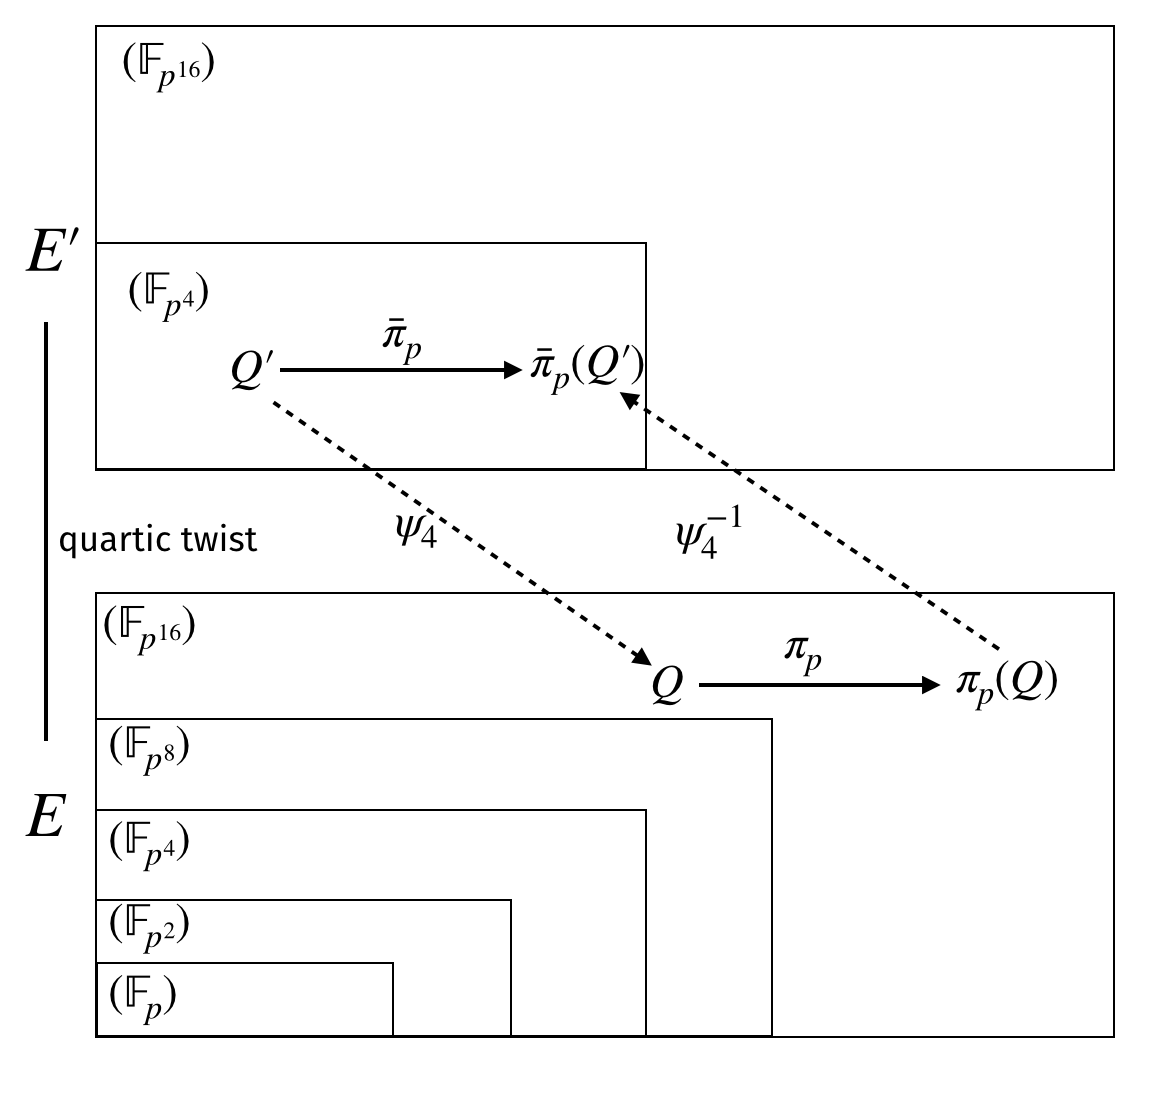
\includegraphics[width=0.7\linewidth]{Figures/skewFMKSS16}
	\caption{Skew Frobenius mapping in \texorpdfstring$\g{2}$ KSS-16 curve.}
	\label{fig:ch:cvma:skewfmkss16}
\end{figure}

%-----------------------------------------
\subsection{Final Exponentiation}
Thanks to the cyclotomic polynomial and the definitions of $r$ and $k$, the exponent $\frac{p^{16}-1}{r}$  broken down into two parts. We have,
$$\frac{p^{16}-1}{r}=(p^8-1)\frac{(p^8+1)}{r}.$$
The first part, $(p^8-1)$ is the simple part of the final exponentiation
because it is easy to be performed thanks to a Frobenius operation, an inversion and a multiplication (in $\mathbb{F}_{p^{16}}$. 
However, it has an important consequence for the computation of the second part of the final exponentiation. 
Indeed, powering $f$, the result of Miller loop,  to the ${p^8-1}$ makes the result unitary \cite{C:ScoBar04}. So during the hard part of the final exponentiation, which consists on computing $f^{\frac{p^8+1}{r}}$), all the elements involved are unitary.
This  simplifies computations, for example, any future inversion can be implemented as a Frobenius operator, more precisely $f^{-1}=f^{p^8}$ which is just a conjugation \cite{C:ScoBar04}, \cite{CHES:StaLen02}. \\
The hard part $\frac{(p^8+1)}{r}$ can be efficiently calculated using Ghammam's et al.'s works \cite{EPRINT:GhaFou16b} addition chain algorithm.\\
In this chapter, we  reduce the number of temporary variables used in the  \cite{EPRINT:GhaFou16b} to calculate $f_1^{857500{\frac{(p^8+1)}{r}}}$, where   $f_1 $ is the result of computing the first part of the final exponentiation. 
The  number $d=857500$, chosen in  \cite{EPRINT:GhaFou16b}  results efficient addition chain calculation  that ultimately helps efficient hard part evaluation.
Alg. \ref{algo_final}  shows the space-optimized final exponentiation. \\
The squaring during hard part computation is the most operation used, it can be efficiently carried out using Granger et Scott  \cite{PKC:GraSco10} cyclotomic squaring. Their method consists of:
%After the easy part evaluation, the $\g3$ element is actually in a cyclotomic subfield. 
Let $A$ be a $\g3$ element that is actually  in a cyclotomic subfield.  So $A = (a_0+a_1\gamma) \in \mF{p}{16}$, it verifies $A^{(p^8+1)}=1$. Therefore,  $(a_0+a_1\gamma) (a_0-a_1\gamma)=1$ or $a_0^2=1+a_1^2\gamma^2 =  1+a_1^2\beta$ can be obtained, where  $\bar{A}=(a_0-a_1\gamma)$ is a conjugate of $A$. 
By using this relation we can obtain the cyclotomic squaring as follows:
\begin{eqnarray}
A^2& = &a_0^2+a_1^2 \beta+2a_0a_1\gamma \nonumber \\
&  = & a_0^2+a_1^2 \beta +((a_0+a_1)^2-a_0^2 -a_1^2)  \gamma\nonumber \\
&=& 1+ a_1^2 \beta + a_1^2 + ((a_0+a_1)^2- 1-a_1^2\beta -a_1^2)\gamma \nonumber \\
&=&  (1+ 2a_1^2 \beta)  + ((a_0+a_1)^2- 1-a_1^2(1+\beta) )\gamma \nonumber 
\end{eqnarray}
Here, only two squaring in $\FPET$ where in normal $\FPSN$ squaring requires 2 multiplications in $\FPET$.

\begin{center}
	\begin{table}[!ht]
				\caption{Final Exponentiation with reduced temporary variables of \cite{EPRINT:GhaFou16b}.}
		\label{algo_final}
		\resizebox{!}{.35\paperheight}{%
		\begin{tabular}{l|c|l}
			\hline
			% after \\: \hline or \cline{col1-col2} \cline{col3-col4} ...
			\textbf{Algorithm 4:}    & Operation &Cost   \\
			%& & \\
			\hline
			\textbf{Input:} $f, u, p, r$&\\
			\textbf{Output:} $f_1^{d{\frac{(p^8+1)}{r}}}$&
			\\
			\textbf{Temp.Var:}$t, t_0,t_1, \cdots, t_{14}$& \\
			\hline
			$f_1 \leftarrow f^{p^8}$, $f_1 \leftarrow f_1*f^{-1}$ &  & \\
			
			\hline
			$t_0 \leftarrow f_1^2$, $t_1 \leftarrow t_0^2$ & $f_1^2, f_1^4$  &$2S_{c16}$\\
			$t_2 \leftarrow f_1^{(u+1)}$, 	$t_3 \leftarrow t_2^{(u+1)}$&$f_1^{(u+1)}$, $f_1^{(u+1)^2}$ &2$E_{u}$\\
			$t_4 \leftarrow t_3*t_1$&$f_1^{(u+1)^2+4} =f_1^B$  &$1M_{p^{16}}$\\
			
			\hline
			$t_5 \leftarrow t_4^{u}$, $ t_6 \leftarrow t_4^5$&$f_1^{uB}$, $f_1^{5B}$&$1E_{u}+1M_{p^{16}}+2S_{c16}$\\
			$t_7 \leftarrow t_1^8$, $t_8 \leftarrow t_7^2$& $f_1^{32}, f_1^{64}$&$4S_{c16}$ \\
			$t_9 \leftarrow t7*t_1^{-1}$, $t_{10} \leftarrow t_9^2$ & $f_1^{28}, f_1^{56}$ &$1M_{p^{16}}+1S_{c16}$\\
			$t_{11} \leftarrow t_5^{u}$, $t_{12} \leftarrow t_{11}^{u}$& $f_1^{u^2B}, f_1^{u^3B}$ &$2E_u$\\
			$t_{13} \leftarrow t_{12}*t_9$& $f_1^{(u^3B+56)}=f_1^A$& $1M_{p^{16}}$\\
			
			\hline
			$t_9 \leftarrow t_{13}^{u}$, $t_2 \leftarrow t_9^{-2}$& $f_1^{uA}, f_1^{-2uA}$&$1E_u+1S_{c16}$\\
			$t_{10} \leftarrow t_6^5$, 	$t_{10} \leftarrow t_{10}^5$&$ f_1^{25B}, f_1^{125B}$&$2M_{p^{16}}+2S_{c16}$\\
			$t_{0} \leftarrow t_2*t_{10}^{-1}$&$f_1^{-2uA-125B}=f_1^{c_2}$&$1M_{p^{16}}$\\
			\hline
			$t_{3} \leftarrow t_0^2$, 	$t_2 \leftarrow t_2^4$ & $f_1^{2c_2}$; $f_1^{-8uA}$ & $3S_{c16}$\\
			$t_2 \leftarrow t_2*t_9$ & $f_1^{-7uA}$& $1M_p^{16}$\\
			$t2 \leftarrow t_2*t_3$& $f_1^{2c_2-7uA} = f_1^{c_6}$& $1M_p^{16}$ \\
			$t_3 \leftarrow t_9^{u}$, $t_6 \leftarrow t_3^{u}$ & $f_1^{u^22A}$; $f_1^{u^3A}$ & $2E_u$\\
			$t_7 \leftarrow t_6^{u}$, $t_{10} \leftarrow t_3^{2}$&$f_1^{u^4}$; $f_1^{2u^2A}$& $1E_u + 1S_{c16}$\\
			\hline
			$t_{9} \leftarrow t_5^5$, $t_{9} \leftarrow t_9^5$&$f_1^{5uB}$;$f_1^{25uB}$&$2M_p^{16}+4S_{c16}$\\
			$t_{4} \leftarrow t_9^3$, $t_{9} \leftarrow t_4*t_9$&$f_1^{75uB}$;$f_1^{100uB}$& $1C_{16}+1M_{p^{16}}$\\
			$t_{10} \leftarrow t_{10}^2$& $f_1^{4u^2A}$&$1S_{c16}$\\
			$t_{14} \leftarrow (t_{10}*t_4)^{-1}$ & $f_1^{-4u^2A-75uB}=f_1^{c_1}$ & $1M_{p^{16}}$\\
			$t_{3} \leftarrow t_{10}*t_3^{-1}$& $f_1^{3u^2A}$&$1M_{p^{16}}$\\
			$t_{3} \leftarrow t_3*t_9$ & $f_1^{3u^2A+100xB}=f_1^{c_5}$ & $1M_{p^{16}}$\\
			$t_{11} \leftarrow t_{11}^5$,$t_{9} \leftarrow t_{11}^2$ & $f_1^{5u^2B}$; $f_1^{10u^2B}$ & $1M_{p^{16}} + 3S_{c16}$ \\
			$t_{4} \leftarrow t_{9}*t_{6}$& $f_1^{u^3A+10u^2B}=f_1^{c_4}$ &$1M_{p^{16}}$\\
			\hline
			$t_{6} \leftarrow t_{6}^2$,$t_{9} \leftarrow t_9^5$& $f_1^{2u^3A}$ $f_1^{50u^2B}$ &$1M_p^{16}+3S_{c16}$\\
			$t_{9} \leftarrow t_{9}*t_{11}$,$t_{9} \leftarrow t_{9}*t_{6}$&$f_1^{55u^2B}$;$f_1^{2u^3A-55u^2B}=f_1^{c_0}$&$2M_p^{16}$\\
			$t_{12} \leftarrow t_{12}^{24}$&$f_1^{24u^3B}$& $1C_{16}+3S_{c16}$\\
			$t_{5} \leftarrow t_{7}^{-1}*t_{12}^{-1}$& $f_1^{-u^4A-24u^3B}$& $1M_p^{16}$\\
			$t_{8} \leftarrow t_{8}^3$, $t_{6} \leftarrow t_{8}*t_{1}$&$f_1^{196}$&$1C_{16}+1M_{p^{16}}$\\
			$t_{7} \leftarrow t_{5}*t_{6}$&$f_1^{-u^4A-24u^3B+196}=F_1^{c_3}$&$1M_{p^{16}}$\\
			$t_{8} \leftarrow t_{13}^{7}$&$f_1^{7A}=f_1^{c_7}$&$2M_{p^{16}}+2S_{c16}$\\
			$t_{1} \leftarrow t_{14}^{p}* t_{7}^{p^3}* t_{3}^{p^5}* t_{8}^{p^7}$&$f_1^{c_1p+c_3p^3+c_5p^5+c_7p^7}$&$3M_{p^{16}}+4(15M)$\\
			$t_{2} \leftarrow t_{0}^{p^2}* t_{2}^{p^6}$&$f_1^{c_2p^2+c_6p^6}$&$1M_{p^{16}}+2(12M)$\\
			$t \leftarrow t_{9}*t_{2}*t_{1}*t_{4}^{p^4}$&$f_1^{d{\frac{(p^8+1)}{r}}}$&$3M_{p^{16}}+1(8M)$\\
			\textbf{return} $t$ & &\\
			\hline
		\end{tabular}
		}
	\end{table}
\end{center}
\vspace{8mm}


Instead of computing the cyclotomic squaring, Karabina has proposed in \cite{Karabina13Squaring} a new method for computing the squaring in the cyclotomic subgroup. This method is called the compressed squaring. It contains two steps, compression where we compute the squaring of the compressed form of an element in the cyclotomic subgroup of $\mathbb{F}_{p^k}$. Then, before performing another operation except the squaring, we have to use the decompression form of the element in question.
In his chapter, Karabina proved that his method is applicable when the extension degree $k=2^a3^b$ with $a, b \in \mathbb{N}$ and  $a, b>0$ and he presented the example of computing the compressed squaring in the cyclotomic subgroup of $\mathbb{F}_{p^{12}}$.
%In this chapter, we are interested in generalizing Karabina's method for  $k=2^a$ and $k=3^b$. In this context, we find the following result.
%\begin{prop}
%For the case of $k=16$, it is not possible to compute the compressed squaring in the cyclotomic subgroup of $\mathbb{F}_{p^{16}}$. Then, this result is generalized when the extension degree $k=2^a$ and $k=3^b$.
%\end{prop}
%%\proof
%Our proof is based on the fact that \dots 
%HERE THE PROOF\\

For this reason, in our work, we consider only the cyclotomic squaring.

The overall optimizations can be seen as the following Alg. \ref{optimal_algo_improved}.

\begin{algorithm}[ht]
	\caption{The improved Optimal-Ate pairing algorithm for KSS-16 curve using CVMA}
	\label{optimal_algo_improved}
	\DontPrintSemicolon
%	
	\KwIn{$u,P\in \g1 \subset E(\FPFR),Q'\in \g2'  \subset E'(\FPFR)$}%input
%	
	\KwOut{$e(\bar{Q'},\bar{P})$} %output

	 Pre-compute $\bar{Q'},\bar{P},y_{P}^{-1}, z^{-2}, z^{-2}\delta$ \Comment*[r]{see Alg. \ref{pre_calc_Algo_cvma_kss16}}
	
	 $f \leftarrow 1, \bar{T'} \leftarrow \bar{Q'}$\;
	 \For{$i = \lfloor \log_2 (u)\rfloor $ {\bf downto} $1$} {
		 $f\leftarrow f^2\cdot \bar{l}_{\bar{T'},\bar{T'}}(\bar{P}) $, $ \bar{T'} \leftarrow [2] \bar{T'} $ \Comment*[r]{apply Alg. \ref{algo_sparse_mul_kss16_cvma} }
		 \If{$u[i]=1$} {
			 $f\leftarrow f\cdot \bar{l}_{\bar{T'},\bar{Q'}}(\bar{P})$, $ \bar{T'} \leftarrow  \bar{T'} + \bar{Q'} $ \Comment*[r]{apply Alg.\ref{algo_sparse_mul_kss16_cvma} to solve \eqref{eq:cvma_kss16_ps_8_add_twist}}}
		 \If{$u[i]=-1$} {
			 $f\leftarrow f\cdot \bar{l}_{\bar{T'},\bar{Q'}}(\bar{P})$, $ \bar{T'} \leftarrow  \bar{T'} - \bar{Q'} $\Comment*[r]{ apply Alg.\ref{algo_sparse_mul_kss16_cvma} to solve \eqref{eq:cvma_kss16_ps_8_add_twist}}}} 
	 $Q_1\leftarrow [u]\bar{Q'}$  \Comment*[r]{here $Q_1 = \bar{T'}$}
	 $Q_2\leftarrow [p]\bar{Q'}$ \Comment*[r]{Skew Frobenius map Sec. \ref{sec:skew_fm_cvmakss16}}
	 $f\leftarrow f\cdot l_{Q_1,Q_2}(\bar{P})$ \Comment*[r]{ Alg.\ref{algo_sparse_mul_kss16_cvma}}
	 $f_t\leftarrow f^{p^3}$   \Comment*[r]{Forbenius map of $p^3$}
	 $f\leftarrow f\cdot f_t$ \Comment*[r]{Alg.\ref{algo_sparse_mul_kss16_cvma}}
	 $f\leftarrow f\cdot l_{\bar{Q'},\bar{Q'}}(\bar{P})$ \Comment*[r]{ Alg.\ref{algo_sparse_mul_kss16_cvma}}
	 $f_1\leftarrow f^{(p^{8}-1)}$  \Comment*[r]{$1I_{p^{16}}+1M_{p^{16}}$}
	 $f\leftarrow f_1^{d\frac{p^{8}+1}{r}}$  \Comment*[r]{ Alg.\ref{algo_final}}
	 {\bf return} $f$\;
\end{algorithm}
%\vspace{6mm}


%------------------------------------------------RESULT----------------------------------------------
\section{Experimental Result Evaluation}\label{sec:4}
This section gives details of the experimental implementation. 
The source code can be found in Github\footnote{\label{source_code_cvma}https://github.com/alaminkhandaker/KSS16-opt-ate}. 
The implemented code is not optimized for any specific platform, rather it is written keeping in mind of scalability with the change of parameters.
The sole purpose of the piece of code is to compare the Optimal-Ate pairing operations between CVMA (this work) and Karatsuba based implementations \cite{INDOCRYPT:KNGDNK17} while applying state-of-art algorithms.

\subsection{Experiment Environment and Assumptions}
Table \ref{table:environemt_cvma_kss16} shows the implementation environment used to evaluate the proposal.  
\renewcommand{\baselinestretch}{1.5}
\begin{table}[ht]
	\centering
		\caption{Computational environment.}
	\label{table:environemt_cvma_kss16}
%	\fontsize{9pt}{9pt}\selectfont
	\resizebox{\columnwidth}{!}{
		\begin{tabular}{|l|c|l|l|c|l|}
			\hline
			CPU{\textsuperscript{*}}                                                                               & Memory & Compiler  & OS               & Language & Library     \\ \hline
			\begin{tabular}[c]{@{}l@{}}Intel(R) Core(TM)\\ i5-6500 CPU @ 3.20GHz\end{tabular} & 4GB    & GCC 5.4.0 & Ubuntu 16.04 LTS & C        & GMP v 6.1.0 \cite{gmp} \\ \hline
		%	\multicolumn{6}{l}{\textsuperscript{*}\footnotesize{Only single core is used from two cores.}}\\
		\end{tabular}
	}
\end{table}
\renewcommand{\baselinestretch}{1.0}

The authors made no attempts to utilize multiple cores of the CPU.
The data type of \verb|mpz_t| of GMP is used to define the big integer in $\FP$.
The code is compiled with \verb|-O3| flag in \verb|gcc|.
To compare the prime field operations of pairing, we assumed that 8 prime field addition $A_p$ in the above environment is almost equivalent to 1 multiplication($M_p$) in $\FP$ with respect of time.
The assumption is based on the average time of 1 million iterations of $A_p$ and $M_p$ of operand size $\approx 334$-bit. 
The authors also found that for the above settings, the assumptions hold in other environments.
TODO %To compare performance with respect to the passage of time,  \path{int clock_gettime(clockid_t __clock_id, struct timespec *__tp)} function is used with clock type \path{CLOCK_MONOTONIC}, that gives time difference as close to wall clock time in milli-second [ms].
The authors also compare the cycles count of the operations, obtained from CPU's  Time Stamp Counter.
It's worth mentioning that none of the time and cycles promise constant output for certain operation in a certain environment due to several operating system factors. 
 
The parameter is chosen according to \cite{EPRINT:BarDuq17}'s suggestion for to make DLP size secure enough against exTNFS \cite{C:KimBar16} as is shown in Table \ref{table:parameters_cvma_kss16}.
The  chosen parameter is twist secure but doesn't guarantee subgroup security.
However, finding both twist secure and subgroup secure parameters with lowest hamming weight can be a matter of time.
\renewcommand{\baselinestretch}{1.5}
\begin{table}[ht]
	%\caption{Selected parameters for 128-bit security level according to  \cite{EPRINT:BarDuq17}}
%	\setlength\tabcolsep{3pt}
	\begin{center}		 
			\caption{Selected parameters for 128-bit security level according to  \cite{EPRINT:BarDuq17}.}
		\label{table:parameters_cvma_kss16}
		\resizebox{\columnwidth}{!}{
			\begin{tabular}{l|l|c|c|c|c|c}
				\hline
				Curve & Integer $u$& HW(u) & $\lfloor\log_2 u \rfloor$ & $\lfloor\log_2 p(u) \rfloor$ & $\lfloor\log_2 r(u) \rfloor$& $\lfloor\log_2 p^k \rfloor$ \\ \hline
				KSS-16 & $u=-2^{33}-2^{32}-2^{13}-2^{11}+2^6+1$ & $6$& $34$ & $334$ & $259$& $5344$\\ \hline
			\end{tabular}
		}
	\end{center}
\end{table}
\renewcommand{\baselinestretch}{1.0}

%-------------------------------------------------------------------------------

\subsection{Result and Analysis}
Table \ref{fp_op_tablel} shows the total number of operations in $\Fp$ for notable finite field operation applied in pairing calculation. 
The negative value refers to the decrements of operations after applying CVMA technique.
As aforementioned, CVMA reduces the number of $A_p$ for multiplications and squaring over the extension field.
Although the Frobenius map in $\FPFR$ is free of cost; however, the Frobenius map in $\FPSN$ in CVMA costs more than  Karatsuba based constructions.
The inversion in $\FPFR$ is costlier in CVMA. 
But in terms of total operation, the CVMA approach shows better performance than Karatsuba approach.
%\renewcommand{\baselinestretch}{1.2}
%%\begin{table}[ht]
%%	\centering
%%	\setlength\tabcolsep{3pt}
%	%\fontsize{10pt}{10pt}\selectfont
%	\begin{adjustbox}{angle=90}
%	\begin{tabular}{l|l|l|l|l|l|l|l|l|}
%		\cline{2-9}
%		& \multicolumn{3}{l|}{CVMA} & \multicolumn{3}{l|}{Karatsuba} & \multirow{2}{*}{\begin{tabular}[c]{@{}l@{}}Increment of $A_p$\\ {[}8$A_p \simeq 1M_p$ in $\Fp${]}\end{tabular}} & \multirow{2}{*}{\begin{tabular}[c]{@{}l@{}}approx \% \\ {[}-ve is  decrement{]}\end{tabular}} \\ 
%		\cline{2-7}
%		& $M_p$ & $A_p$ & $I_p$ & $M_p$ & $A_p$ & $I_p$ &  &  \\ \hline
%		\multicolumn{1}{|l|}{$\FPFR$ inversion} & 16 & 26 & 1 & 14 & 29 & 1 & 13 & 9.2 \\ \hline
%		\multicolumn{1}{|l|}{$\FPFR$ multiplication} & 9 & 22 &  & 9 & 29 &  & -7 & -6.9 \\ \hline
%		\multicolumn{1}{|l|}{$\FPFR$ squaring} & 6 & 14 &  & 6 & 24 &  & -10 & -13.9 \\ \hline
%		\multicolumn{1}{|l|}{$\FPET$ inversion} & 46 & 109 & 1 & 44 & 140 & 1 & -15 & -3 \\ \hline
%		\multicolumn{1}{|l|}{$\FPET$ multiplication} & 27 & 93 &  & 27 & 108 &  & -15 & -4.6 \\ \hline
%		\multicolumn{1}{|l|}{$\FPET$ squaring} & 18 & 78 &  & 18 & 80 &  & -2 & -0.9 \\ \hline
%		\multicolumn{1}{|l|}{$\FPSN$ inversion} & 136 & 466 & 1 & 134 & 525 & 1 & -43 & -2.7 \\ \hline
%		\multicolumn{1}{|l|}{$\FPSN$ multiplication} & 81 & 326 &  & 81 & 365 &  & -39 & -3.8 \\ \hline
%		\multicolumn{1}{|l|}{$\FPSN$ squaring} & 54 & 240 &  & 54 & 258 &  & -18 & -2.6 \\ \hline
%		\multicolumn{1}{|l|}{$\FPSN$ Frobenius} & 27 & 66 &  & 14 &  &  & 170 & 151.7 \\ \hline
%		\multicolumn{1}{|l|}{\begin{tabular}[c]{@{}l@{}}$\FPSN$ skew Frob.\end{tabular}} & 18 & 44 &  & 8 &  &  & 124 & 193.8 \\ \hline
%	\end{tabular}
%	\caption{Operation count in $\FP$ for extension field operations used in pairing}
%	\label{fp_op_tablel}
%\end{adjustbox}
%\end{table}
%\renewcommand{\baselinestretch}{1.0}
\begin{sidewaystable}
	\centering
		\caption{Operation count in $\FP$ for extension field operations used in pairing.}
		\label{fp_op_tablel}
	\begin{tabular}{l|l|l|l|l|l|l|l|l|}
	\cline{2-9}
	& \multicolumn{3}{l|}{CVMA} & \multicolumn{3}{l|}{Karatsuba} & \multirow{2}{*}{\begin{tabular}[c]{@{}l@{}}Increment of $A_p$\\ {[}8$A_p \simeq 1M_p$ in $\Fp${]}\end{tabular}} & \multirow{2}{*}{\begin{tabular}[c]{@{}l@{}}approx \% \\ {[}-ve is  decrement{]}\end{tabular}} \\ 
	\cline{2-7}
	& $M_p$ & $A_p$ & $I_p$ & $M_p$ & $A_p$ & $I_p$ &  &  \\ \hline
	\multicolumn{1}{|l|}{$\FPFR$ inversion} & 16 & 26 & 1 & 14 & 29 & 1 & 13 & 9.2 \\ \hline
	\multicolumn{1}{|l|}{$\FPFR$ multiplication} & 9 & 22 &  & 9 & 29 &  & -7 & -6.9 \\ \hline
	\multicolumn{1}{|l|}{$\FPFR$ squaring} & 6 & 14 &  & 6 & 24 &  & -10 & -13.9 \\ \hline
	\multicolumn{1}{|l|}{$\FPET$ inversion} & 46 & 109 & 1 & 44 & 140 & 1 & -15 & -3 \\ \hline
	\multicolumn{1}{|l|}{$\FPET$ multiplication} & 27 & 93 &  & 27 & 108 &  & -15 & -4.6 \\ \hline
	\multicolumn{1}{|l|}{$\FPET$ squaring} & 18 & 78 &  & 18 & 80 &  & -2 & -0.9 \\ \hline
	\multicolumn{1}{|l|}{$\FPSN$ inversion} & 136 & 466 & 1 & 134 & 525 & 1 & -43 & -2.7 \\ \hline
	\multicolumn{1}{|l|}{$\FPSN$ multiplication} & 81 & 326 &  & 81 & 365 &  & -39 & -3.8 \\ \hline
	\multicolumn{1}{|l|}{$\FPSN$ squaring} & 54 & 240 &  & 54 & 258 &  & -18 & -2.6 \\ \hline
	\multicolumn{1}{|l|}{$\FPSN$ Frobenius} & 27 & 66 &  & 14 &  &  & 170 & 151.7 \\ \hline
	\multicolumn{1}{|l|}{\begin{tabular}[c]{@{}l@{}}$\FPSN$ skew Frob.\end{tabular}} & 18 & 44 &  & 8 &  &  & 124 & 193.8 \\ \hline
\end{tabular}
\end{sidewaystable}

Then, in Table \ref{miller_op_table} we compare   Miller algorithm with CVMA with Miller algorithm with Karatsuba  with respect to operation count.

\renewcommand{\baselinestretch}{1.2}
\begin{table}[ht]
	\centering
		\caption{Miller's algorithm (MA) operation comparison with respect to $\FP$ addition.}
	\label{miller_op_table}
	%	\fontsize{10pt}{10pt}\selectfont
	\resizebox{\columnwidth}{!}{
	\begin{tabular}{l|l|l|l|l|l|l|l|l|}
		\cline{2-9}
		& \multicolumn{3}{l|}{CVMA} & \multicolumn{3}{l|}{Karatsuba} & \multirow{2}{*}{\begin{tabular}[c]{@{}l@{}}Increment\\ of $A_p$\end{tabular}} & \multirow{2}{*}{\begin{tabular}[c]{@{}l@{}}approx \%\end{tabular}}  \\
		\cline{1-7}
		\multicolumn{1}{|l|}{Operations} & $M_p$ & $A_p$ & $I_p$ & $M_p$ & $A_p$ & $I_p$ &  &  \\ \hline
		\multicolumn{1}{|l|}{MA } & 6679 & 23663 & 41 & 6578 & 27194 & 41 & -2723 & -3.4 \\ \hline
		\multicolumn{1}{|l|}{MA pre-com} & 98 & 212 & 2 & 94 & 280 & 2 & -36 & -3.5 \\ \hline
		%		\multicolumn{1}{|l|}{ML old param} &  &  &  & 6638 & 27448 & 41 &  &  \\ \hline
		%		\multicolumn{1}{|l|}{ML Indocrypt} &  &  &  & 7209 &  &  &  &  \\ \hline
		%		\multicolumn{1}{|l|}{ML Sylvain estm.} &  &  &  & 7534 &  &  &  &  \\ \hline
	\end{tabular}
}
\end{table}
\renewcommand{\baselinestretch}{1.0}

In the following Table \ref{final_expo_tab} we compare  the final exponentiation with CVMA with Miller algorithm with Karatsuba  with respect to operation count.

\renewcommand{\baselinestretch}{1.2}
\begin{table}[ht]
	\centering
	%	\fontsize{10pt}{10pt}\selectfont
%	\setlength\tabcolsep{4pt}
	\caption{Comparison in terms of operation count for Final exponentiation (FE).}
	\label{final_expo_tab}
\resizebox{\columnwidth}{!}{
\begin{tabular}{l|l|l|l|l|l|l|}
	\cline{2-7}
	& \multicolumn{2}{l|}{CVMA} & \multicolumn{2}{l|}{Karatsuba} & \multirow{2}{*}{Increment of $A_p$} & \multirow{2}{*}{approx \%} \\ \cline{2-5}
	& $M_p$ & $A_p$ & $M_p$ & $A_p$ &  &  \\ \hline
	\multicolumn{1}{|l|}{Pseudo 8-sparse multiplication} & 54 & 205 & 54 & 229 & -24 & -3.6 \\ \hline
\end{tabular}
}
\end{table}
\renewcommand{\baselinestretch}{1.0}

The Miller's algorithms proposed pre-computation cost is negligible compared to the rest of the computation.
The Karatsuba based implementation takes 101 less $\Fp$ multiplication than CVMA in Miller's algorithm.
However, such advantage is overtaken by the number of reduced addition in CVMA~\index{CVMA} compared to Karatsuba.
The $3.4\%$ improvement is seemingly very insignificant in terms of 1 pairing. 
However, a real pairing-based protocol requiring multiple pairings can be benefited from it.
% \textcolor{red}{However, a real pairing-based protocol requiring multiple pairings can be benefited from it. \textbf{WHY?? Explain}}

Table \ref{time_com_pairing} shows  execution time in millisecond (rounded 2 decimal places) and cycle counts for Optimal-Ate pairing implementation for the Table \ref{table:environemt_cvma_kss16} settings. 
The main purpose of this execution time comparison is to show that the theoretic optimization also reflects in the real implementation.
However, the implementation doesn't guarantee constant time operation which is crucial in the context of the side-channel attack.
The negative value refers to CVMA's efficiency over Karatsuba based implementation. 
The cycle counts are almost coherent with the time performances.
The execution time  also binds with the respective operation counts of Table \ref{miller_op_table}, \ref{final_exp_op_count_table}.
%Since the operation is time negligible compared to Miller' loop we over looked this step.
The total pairing time is significantly influenced by the hard part of final exponentiation. 
It may seem confusing that $0.7\%$ reduction of operation count for the FE hard part in CVMA, results in  relatively more faster execution time.
However, we relate this irregularity to cyclotomic squaring operation.
Since towering is involved, therefore, the extension field operations are implemented in top-down order.
Therefore, in CVMA, the $\FPET$ squaring for cyclotomic squaring operation, calls $\FPFR$ squaring; which is more efficient than the Karatsuba counterpart (Table \ref{fp_op_tablel}).
The further time-profile investigation finds that  the number of times GMP library calls its  memory allocation/reallocation impacts in the execution time.

\renewcommand{\baselinestretch}{1.2}
\begin{table}[ht]
	\centering
	%	\fontsize{10pt}{10pt}\selectfont
%	\setlength\tabcolsep{4pt}
	\caption{Comparison in terms of operation count for Final exponentiation (FE).}
\label{final_exp_op_count_table}
\resizebox{\columnwidth}{!}{
	\begin{tabular}{l|l|l|l|l|l|l|l|l|}
		\cline{2-9}
		& \multicolumn{3}{l|}{CVMA} & \multicolumn{3}{l|}{Karatsuba} & \multirow{2}{*}{\begin{tabular}[c]{@{}l@{}}Increment \\of $A_p$\end{tabular}} & \multirow{2}{*}{\begin{tabular}[c]{@{}l@{}}approx \%\end{tabular}} \\
		\cline{1-7} 
		\multicolumn{1}{|l|}{Operations} & $M_p$ & $A_p$ & $A_{ui}$ &  $M_p$ & $A_p$ & $A_{ui}$ &  &  \\ \hline
		\multicolumn{1}{|l|}{Final exp. {[}hard{]}} & 19134 & 93933 & 2744 & 19102 & 96129 & 686& -1796 & -0.7\\ \hline
		\multicolumn{1}{|l|}{Final exp. {[}easy{]}} & 217 & 792 &  & 215 & 890 & & -82 & -3.1 \\ \hline
	\end{tabular}
}
\end{table}

\renewcommand{\baselinestretch}{1.0}

\renewcommand{\baselinestretch}{1.2}
\begin{table}[ht]
	\centering
%	\setlength\tabcolsep{4pt}
\caption{Time comparison in  millisecond [ms] of CVMA vs Karatsuba based implementation of Pseudo 8-sparse Optimal-Ate.}
\label{time_com_pairing}
		\resizebox{\columnwidth}{!}{
	\begin{tabular}{l|l|l|l|l|l|l|}
	\cline{2-7}
	& \multicolumn{2}{l|}{CVMA} & \multicolumn{2}{l|}{Karatsuba} & \multicolumn{2}{l|}{\begin{tabular}[c]{@{}l@{}}Increment in \%\\ {[}-ve refers decrement{]}\end{tabular}} \\ \cline{2-7} 
	& $\approx$ Time {[}ms{]} & Cycles & $\approx$ Time {[}ms{]} & Cycles & Time & Cycles \\ \hline
	\multicolumn{1}{|l|}{\begin{tabular}[c]{@{}l@{}}Pairing pre-\\computation\end{tabular}} & 0.05 & 159161 & 0.05 & 156660 & 0 & 1.6 \\ \hline
	\multicolumn{1}{|l|}{Miller's algo.} & 2.23 & 7125491 & 3.45 & 11010338 & -35.4 & -35.3 \\ \hline
	\multicolumn{1}{|l|}{FE {[}easy{]}} & 0.12 & 378786 & 0.13 & 413408 & -7.7 & -8.4 \\ \hline
	\multicolumn{1}{|l|}{FE {[}hard{]}} & 7.13 & 22765766 & 10.18 & 32507719 & -30.0 & -30.0 \\ \hline
	\multicolumn{1}{|l|}{Total} & 9.53 & 30429204 & 13.81 & 44088125 & -31.0 & -31.0 \\ \hline
\end{tabular}
}
\end{table}
\renewcommand{\baselinestretch}{1.0}

%-----------------------------------------------------------------------------
\section{Conclusion and Future Work}\label{sec:5}
This chapter shows several improvement ideas for Optimal-Ate pairing in the less studied KSS-16 curve while revisiting \cite{INDOCRYPT:KNGDNK17} to find more efficient Miller's algorithm implementation technique for Optimal-Ate pairing
\begin{itemize}
	\item applied combination of normal basis  and polynomial basis for $\FPSN$ extension field operation.
%	\item for $\FPFR$ extension field to adapt CVMA and polynomial basis for rest of the extension field operations. 
\item	The selling point for of CVMA in this work is $\FPFR$ extension field operation. 
	It requires fewer $\FP$ additions than its Karatsuba counterparts. 
	However, Inversion and Frobenius map for the $\FPSN$ is still expensive for the applied towering.
	\item The authors optimized inversion operation cost for CVMA approach.
	\item  Optimized the pseudo 8-sparse multiplication for CVMA, which becomes $3.6\%$ efficient than the similar method presented in IndoCrypt'17 \cite{INDOCRYPT:KNGDNK17}.
	\item  The final exponentiation by Ghammam et al \cite{EPRINT:GhaFou16b} is more memory-optimized now. 
\end{itemize}
The main drawback of this CVMA setting is the inversion in $\FPFR$ and Frobenius map in $\FPSN$.
As a future improvement, we would like to find settings which can overcome these obstacles. 
The implementation and execution time given here is a comparative purpose. It can be more optimized by careful low-level prime field implementation.

%  \subsection{Contribution Summary}
%Finding efficiently computable underlying finite field arithmetic is one of the major bottlenecks for faster pairing operation.
%In this chapter, we exhibit efficiently computable extension field operation for Optimal-Ate pairing in Kachisa-Schaefer-Scott curve of embedding degree 16. 
%The recent suggestion of escalating parameter's size by Barbulescu and Duquesne due to improved Kim and Barbulescu's new number field sieve (exTNFS) have taken into account while selecting the parameter for 128-bit  level AES security.
%The authors revisited their idea of $\PESM$ for line evaluation in Miller's algorithm presented in IndoCrypt'2017, with more efficient base field arithmetic by applying cyclic vector multiplication algorithm (CVMA) in the $\FPFR$ extension field.
%To compare the complexity of this work with the previous one,
%the base extension field $\FPFR$ is constructed in two different bases.
%Moreover, the state-of-the-art final exponentiation algorithm is optimized with cyclotomic squaring technique. 
%The comparative results find that the CVMA has a clear advantage over Karatsuba based operation.
